\chapter{W boson pT spectrum}
    \chapterprecishere{
        ``Potentielle citation sans aucun rapport avec le sujet"\par\raggedleft--- \textup{Personne inconnue}, contexte à déterminer
    }

\section{Unfolding}
The measured W $p_T$ spectrum is subject to various detector effects (finite resolution and acceptance, reconstruction efficiency, etc.) that distort the true underlying spectrum. Mathematically, the unfolding problem is an integral equation of the following form:
\begin{equation}
	\int K(x,y)\cdot f(x)dx = g(y),
\end{equation}
where we seek the function $f(x)$ assuming that $g(y)$ and the kernel $K(x,y)$ are known \cite{Schmitt:2016orm}. The function $g(y)$ is convoluted (or folded) with the kernel hence the name of the problem. In experimental physics it is more common to use binned distributions instead of continuous functions: 
\begin{equation}
\sum_{i} \textbf{R}_{ij}\cdot \textbf{T}_i + \textbf{B}_j = \textbf{D}_j,
\end{equation}
with $\textbf{D}$, $\textbf{T}$ and $\textbf{B}$ being vectors that represent detector-level (measured), truth and background distributions respectively; each vector has $n$ components that represent the bins in the corresponding distribution. The response matrix $\textbf{R}$ represents bin-to-bin migrations caused by the detector effects. \\
The response matrix is usually obtained through \gls{mc} simulation, along with the corrections for the fiducial volume acceptance and efficiency. Each event is simulated on the truth and reconstructed levels, this means that element $R_{il}$ of the migration matrix contains events that pass both reconstruction and truth cuts (R\&T) and would go to bin $i$ of the truth distribution and to bin $j$ of the reconstructed distribution. Detector acceptance for bin $i$ is defined as the ratio $A_i=\sum_j R{ij}/T_i$. Similarly the reconstruction efficiency for bin $j$ is defined as the ratio $\epsilon_j=\sum_i R{ij}/D_j$.
The underlying distribution estimate is presented in the following way:
\begin{equation}
\sum_{i} \textbf{V}_{ij}\cdot (\textbf{D}_i - \textbf{B}_i) = \textbf{U}_j,
\end{equation}
 where $U$ vector provides the underlying distribution estimate and $V$ is the unfolding transformation matrix.\\
 There exist a diverse variety of methods to obtain the unfolding transformation. In the current analysis a Bayesian iterative method is used \cite{unfolding1}, \cite{unfolding2}. The method allows to obtain the unfolding transformation provided that the response matrix, acceptance and efficiency corrections are known and the number of iterations is given. The number of iterations as well as the unfolded distribution binning are adjusted in order to minimize the unfolding bias and keep the uncertainty below the designated level.

\begin{figure}[htpb]
	\centering
	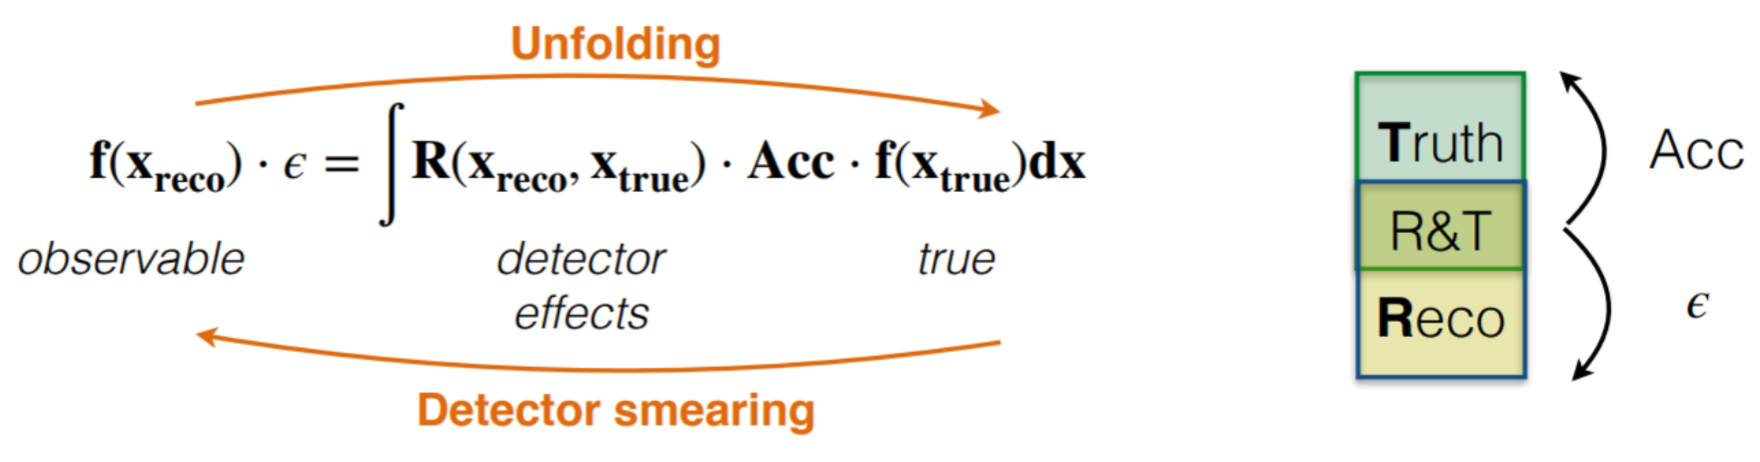
\includegraphics[width=\textwidth,keepaspectratio]{unfold}
	\caption[Unfolding]{Schematic description of the unfolding procedure.}
	\label{fig::unfolding}
\end{figure}

\section{Uncertainties propagation}
The detector-level uncertainties breakdown for the \pt distribution are presented here. Uncertainties breakdown for the rest of the observables are listed in Appendix A. \\
These uncertainties now have to be propagated to the unfolded level. 
\subsection{Statistical uncertainty propagation using Bootstrap method}
Bootstrap is a computer-based method of dataset parameters estimate and propagation using the analysis distribution resampling. In particular bootstraping used for the propagation of statistical uncertainties. \\
Both data and MC-simulated datasets have limited number of events, hence the statistical uncertainties due to fluctuations. In order to estimate the statistical uncertainty a number of pseudo-data sets is generated for both data and \gls{mc} where each event is assigned a random weight $w$:
\begin{equation}
w = \mathcal{P}(n,1),
\end{equation}
where $n$ is a random number generated with Poisson distribution with mean $\lambda=1$, value $\mathcal{P}(n,1)$ is a Poissonian probability of observing n events while expecting an average of 1 event.\\
The boostrapping defined in this way allows to take into account the correlated effect of statistical fluctuations across all observables and distributions in the analysis. For the determination of statistical uncertainty of the unfolded spectrum 400 bootstrap samples were generated.
In both data and MC cases the statistical uncertainty is estimated by composing the covariant matrix $C_{kl}^{\textrm stat}$:
\begin{equation}
C_{kl}^{\textrm stat} = \frac{1}{N_{bs}-1} \sum_{\alpha=1}^{N_{bs}} (U^\alpha_k-\langle{U}_k\rangle) \, (U^\alpha_l-\langle{U}_l\rangle),
\label{eq:covexpr}
\end{equation}
where $N_{bs}$ is the number of the Bootstrap toys used, vector $U$ stands for the varied underlying distribution, $\langle{U}_k\rangle$ is the average underlying distribution. However, the variation is performed in a different way for Data and MC:
 \begin{equation*}
U_j^{\alpha,(MC)} = V_{ij}^\alpha \sum_{i} (D_i - B_i),
 \end{equation*}
  \begin{equation*}
U_j^{\alpha,(Data)}  = V_{ij} \sum_{i} (D_i^\alpha - B_i).
 \end{equation*}
 In the MC case it is the response matrix $V^\alpha$ to be varied ($\alpha$ index corresponds to the variation number), whereas in Data the toys are obtained by varying the measured distribution $D^\alpha_i$. The statistical uncertainty for both cases is defined as:
 \begin{equation}
 \delta U_k = \sqrt{C_{kk}^{\textrm stat}}.
 \end{equation}
\subsection{Systematic uncertainty propagation}
Systematic uncertainties are broken down into a number of uncorrelated uncertainty sources, which include signal and background modelling uncertainties, calibration and efficiency uncertainties, physics modelling uncertainties. The systematic variations used for uncertainty estimate on the detector level are propagated to the level of underlying distribution in two different ways. For the background uncertainties:
 \begin{equation*}
U_j^{a} = V_{ij}\sum_{i} (D_i - B^a_i),
\end{equation*}
total background estimate $B^a_i$ is varied in luminosity and cross-section of every back-ground (index $a$ numbers the sources of uncertainty). For other sources of systematic uncertainty:
 \begin{equation*}
U_j^{a} = V_{ij}^a \sum_{i} (D_i - B_i),
\end{equation*}
response matrix variation is created. The corresponding covariance matrix is defined as:
 \begin{equation*}
C_{kj}^{a} = \delta U^a_k \delta U^a_l,
\end{equation*}
where the deltas are $\delta U^a_k=U^a_k-U^{Nom}_k$.
The total covariance matrix is calculated as a sum:
\begin{equation}
C_{kl}^{\textrm tot} = C_{kl}^{\textrm stat,Data} + C_{kl}^{\textrm stat,MC} + \sum_a C_{kl}^a.
\end{equation}	
\subsection{Unfolded uncertainty breakdown}
Figures \ref{fig:reco_sys_bkd_elec}, \ref{fig:reco_sys_bkd_muons}, contain the systematic uncertainties breakdown for electron and muon channels for the reconstructed level distributions for 5 and 13 TeV. Similarly figures \ref{fig:unf_sys_bkd_elec}, \ref{fig:unf_sys_bkd_muons} contain unfolded-level uncertainties. \\
At the detector level the designated level of uncertainty of below 1\% is preserved up to 25 \gev{} for 5 \tev{} datasets and up to 50 \gev{} for 13 \tev{} samples in every channel. An increased role of background uncertainty is observed at 13 \tev{} due to the significantly higher cross-sections of diboson and top-antitop backgrounds.
The scale and hierarchy of uncertainties are preserved at the unfolded level. 

\begin{figure}[h]
	\centering
	{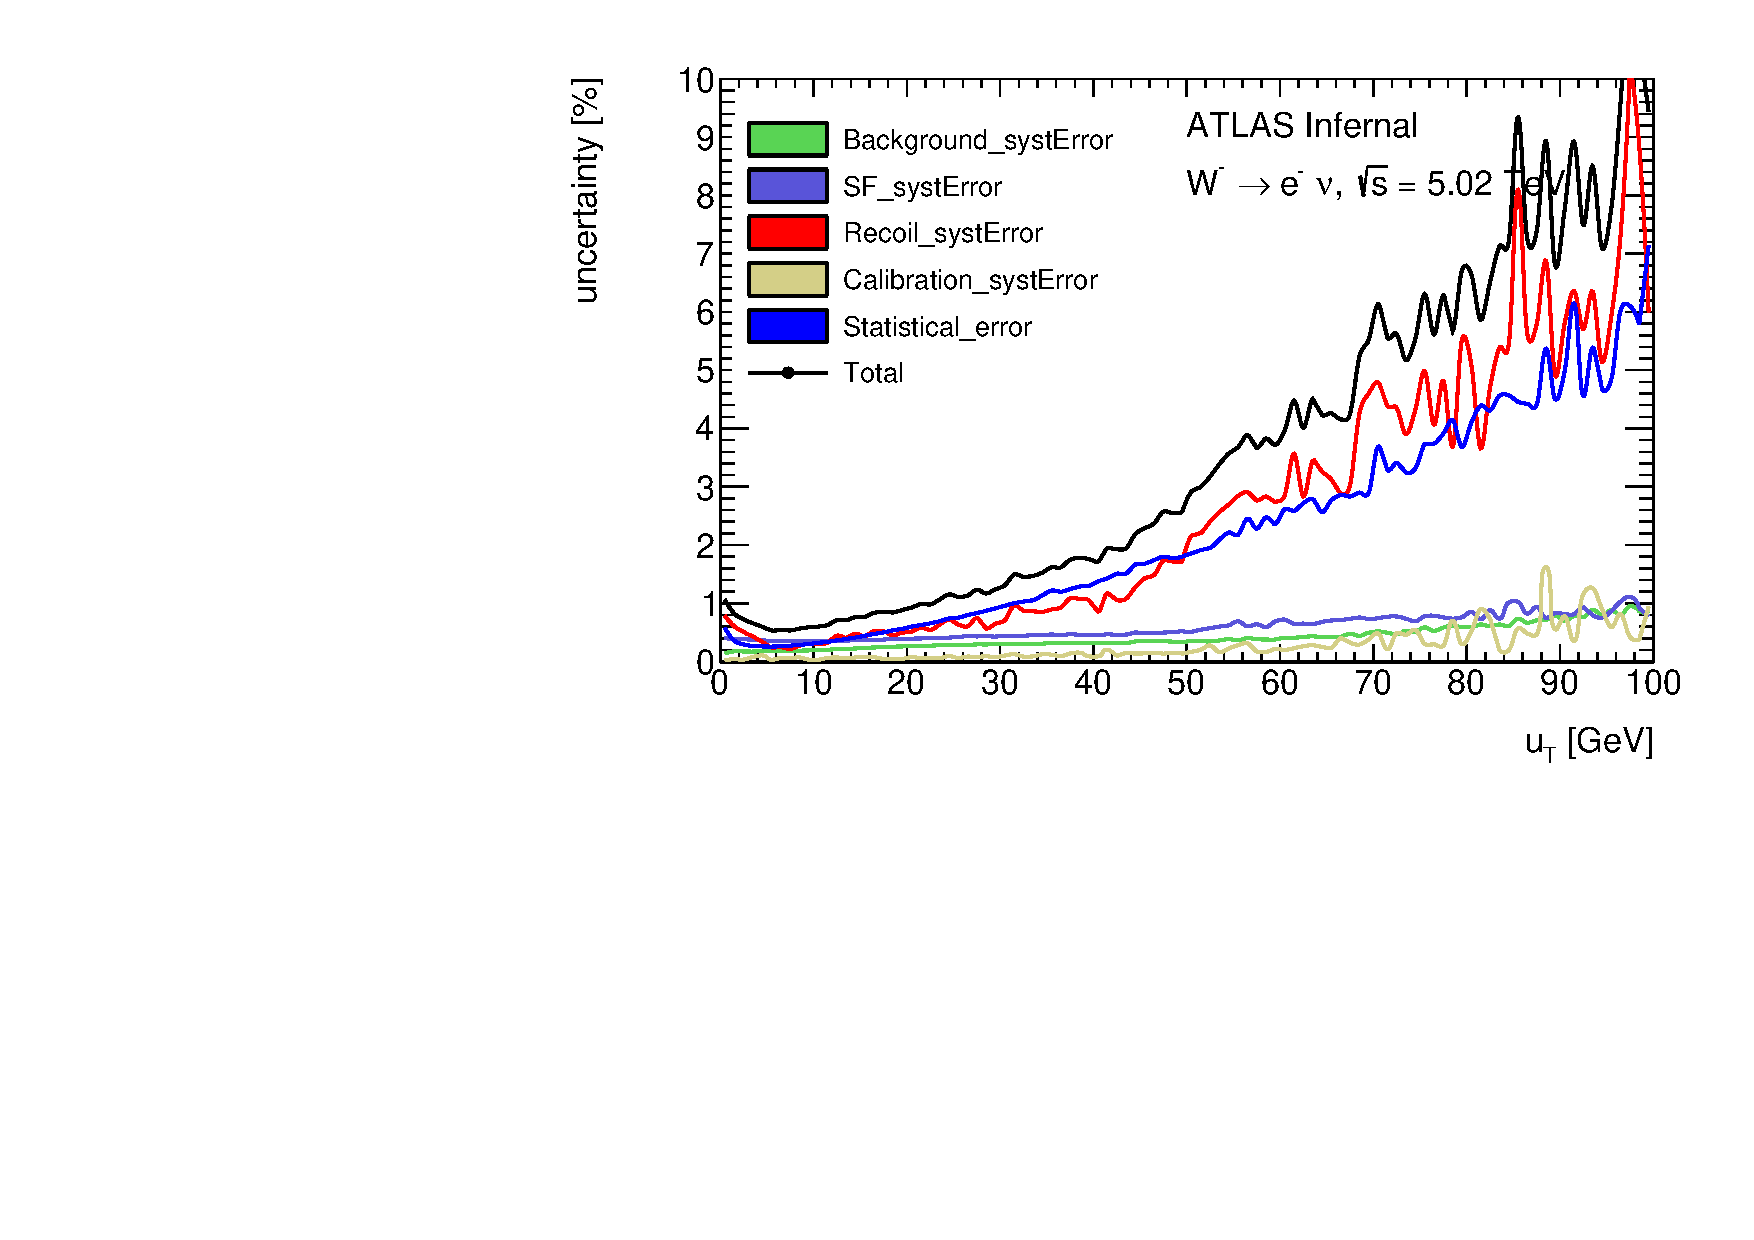
\includegraphics[width=.49\textwidth]{errors_WpT_Reco_cut7_minusenu_5TeV_test1}}
	{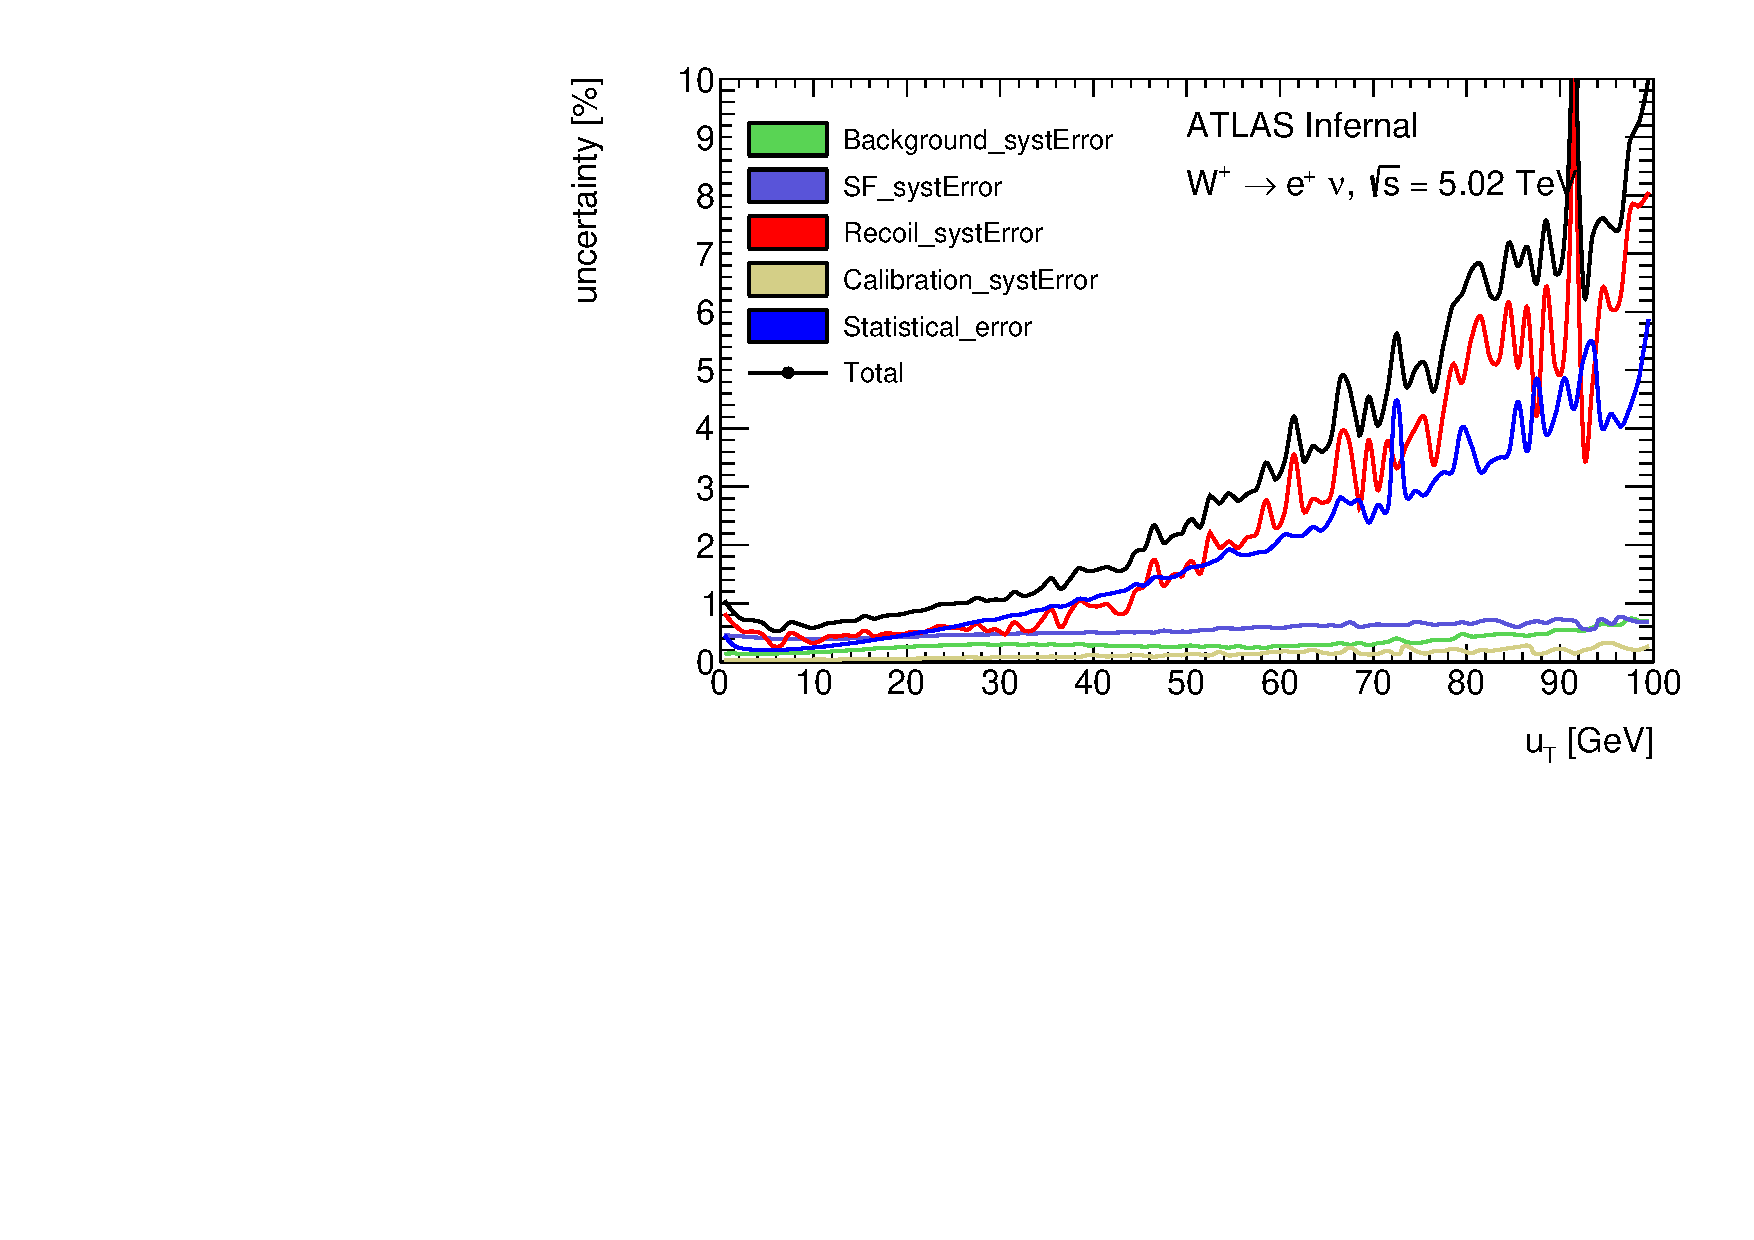
\includegraphics[width=.49\textwidth]{errors_WpT_Reco_cut7_plusenu_5TeV_test1}} \\
	{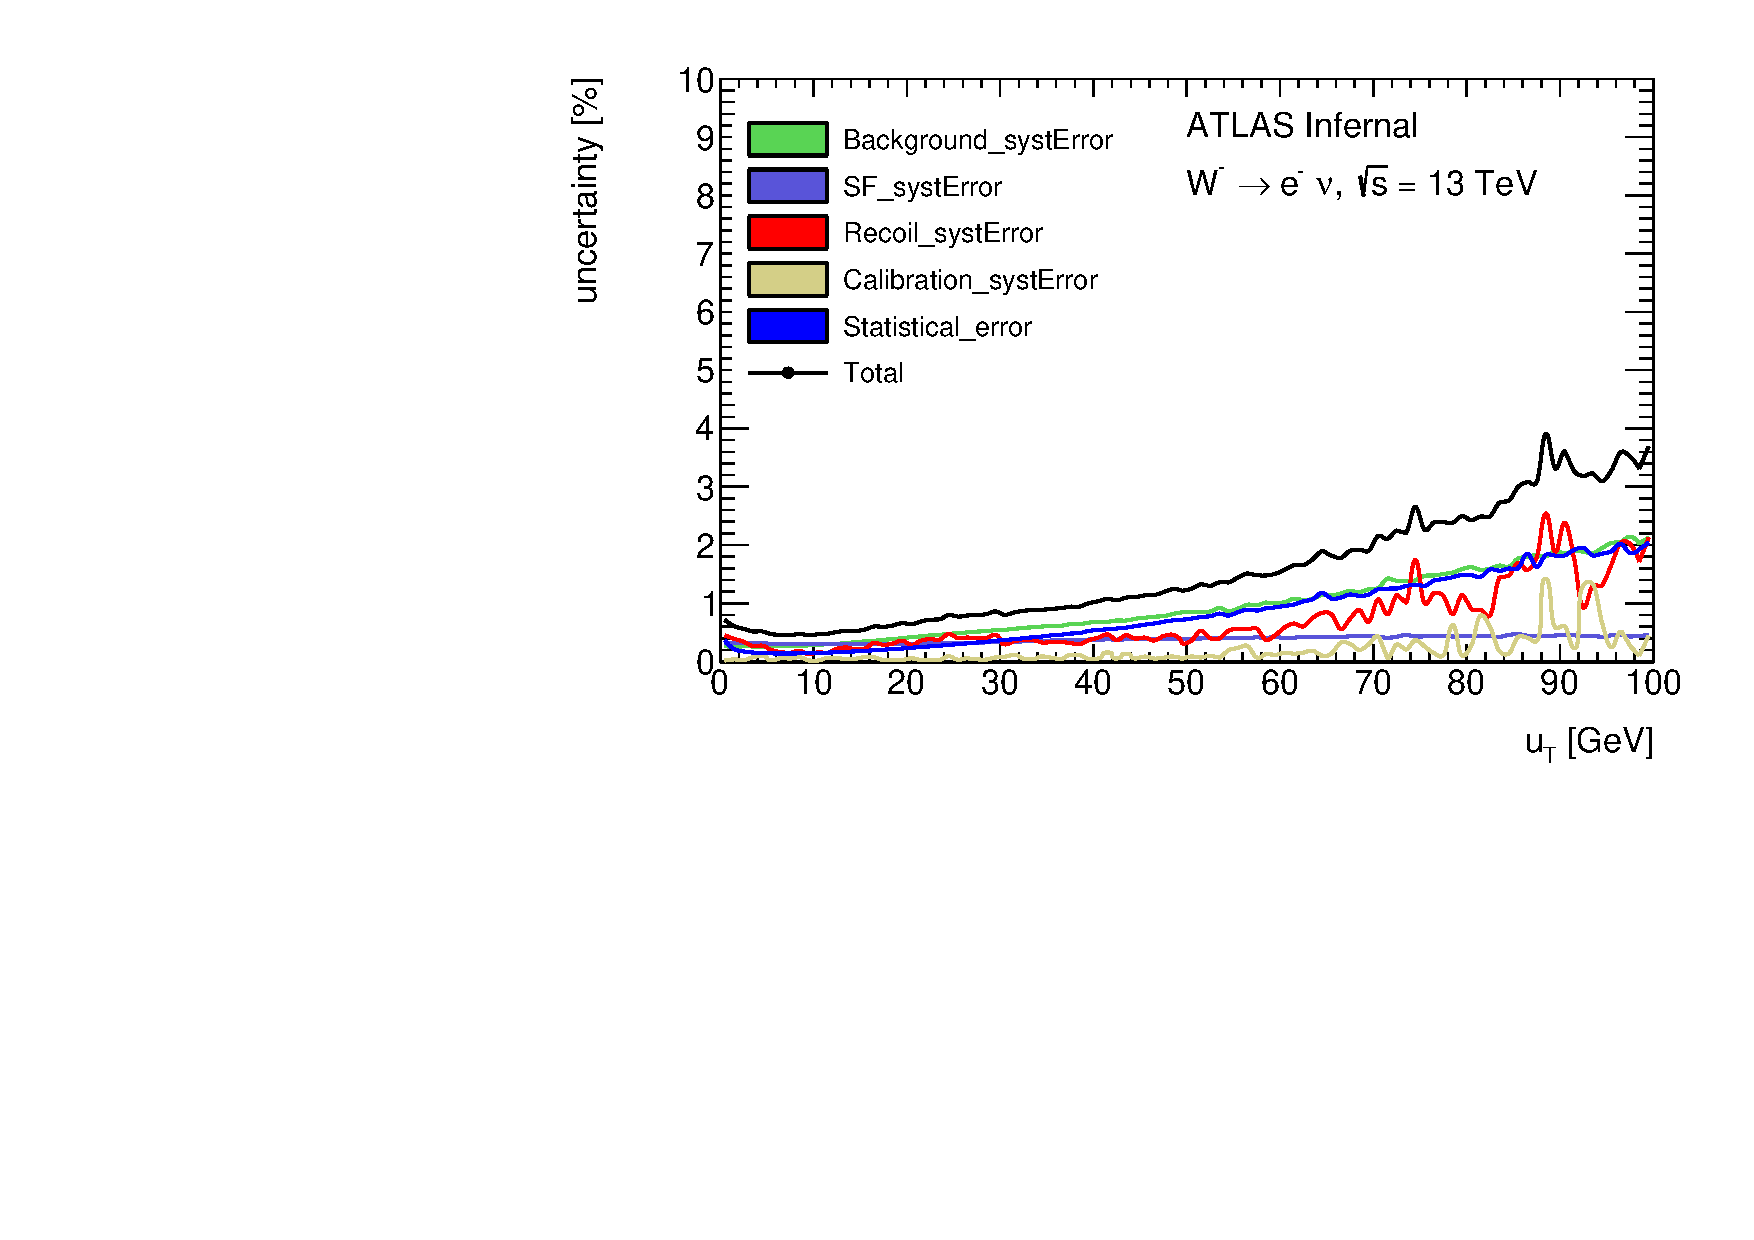
\includegraphics[width=.49\textwidth]{errors_WpT_Reco_cut7_minusenu_13TeV_test1}}
	{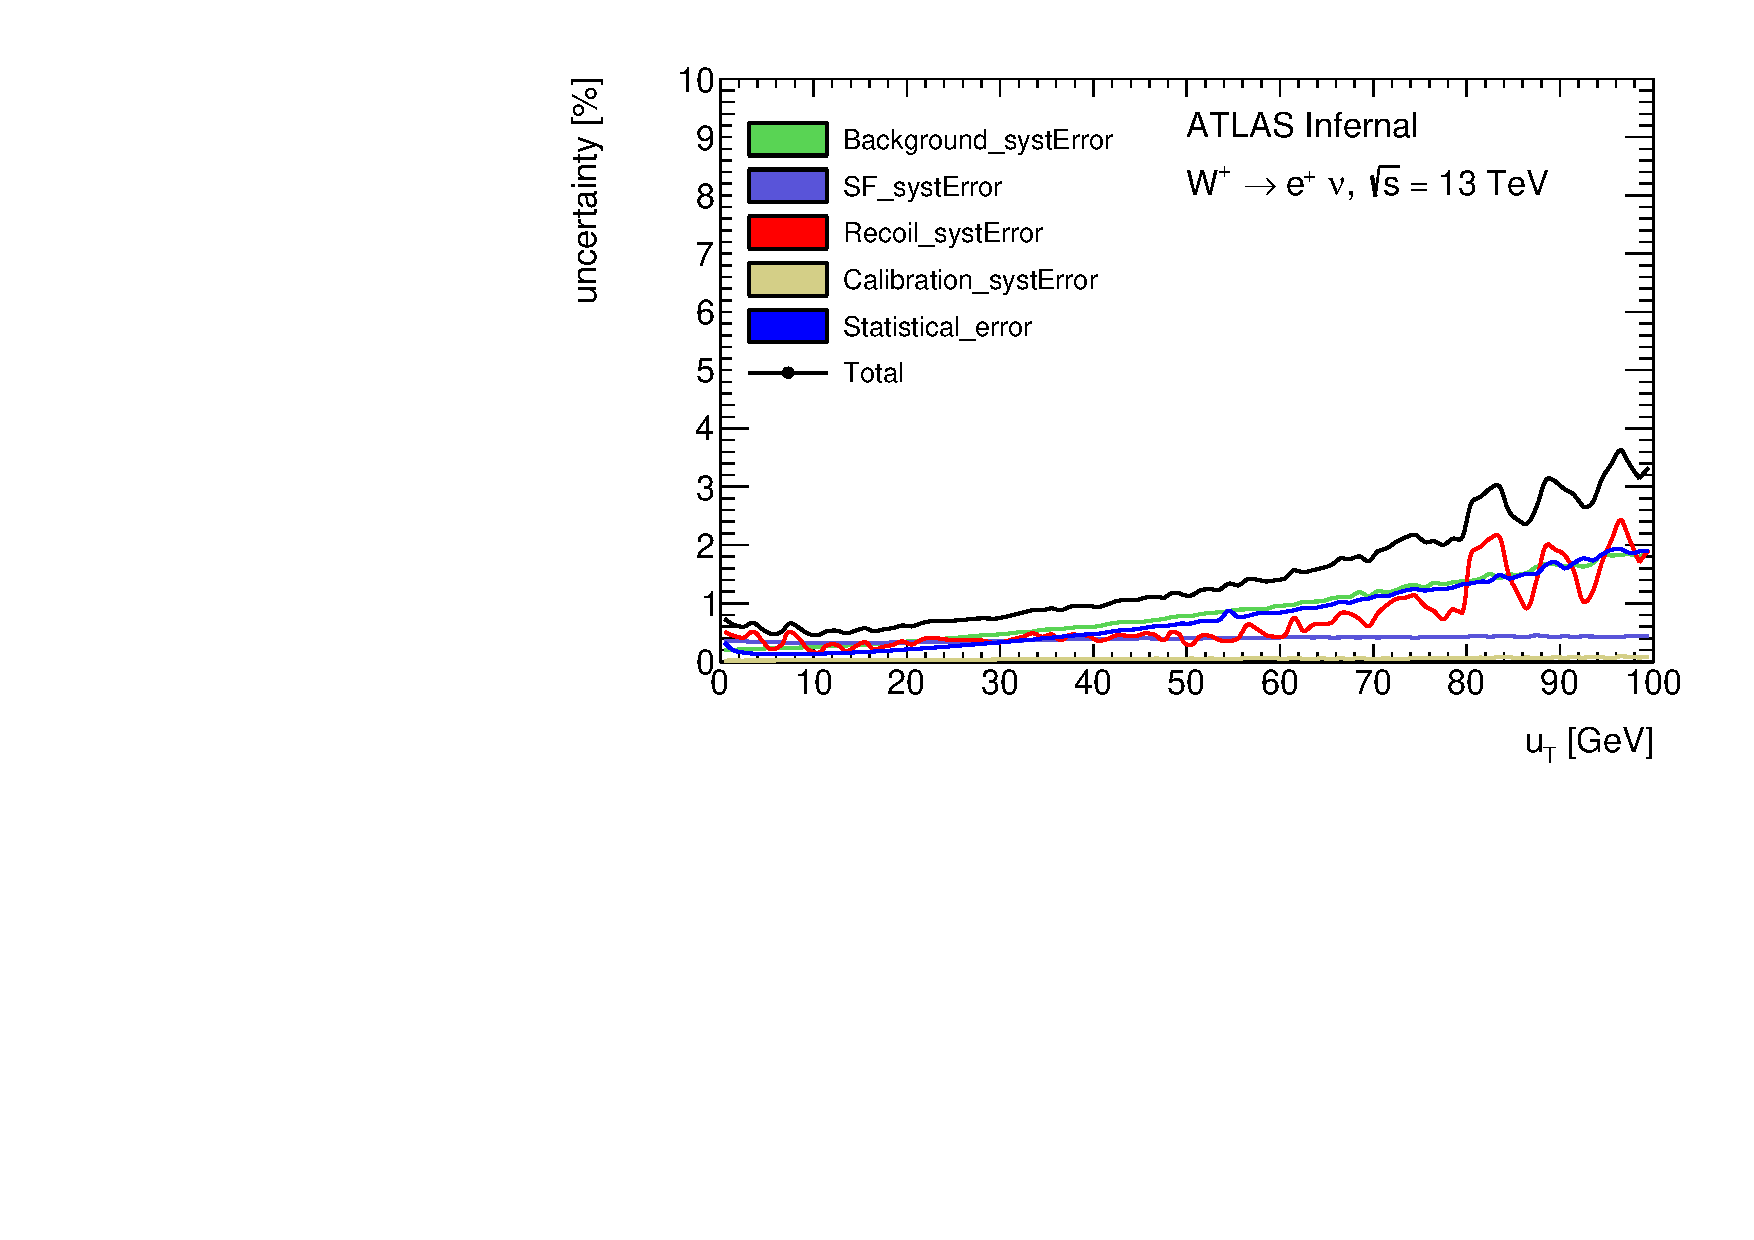
\includegraphics[width=.49\textwidth]{errors_WpT_Reco_cut7_plusenu_13TeV_test1}}
	
	\caption{ Breakdown of systematic uncertainties for 5 (a,b) and 13 (c,d) TeV in the electron channel at the reconstructed level}
	\label{fig:reco_sys_bkd_elec}
\end{figure}

\begin{figure}[h]
	\centering
	{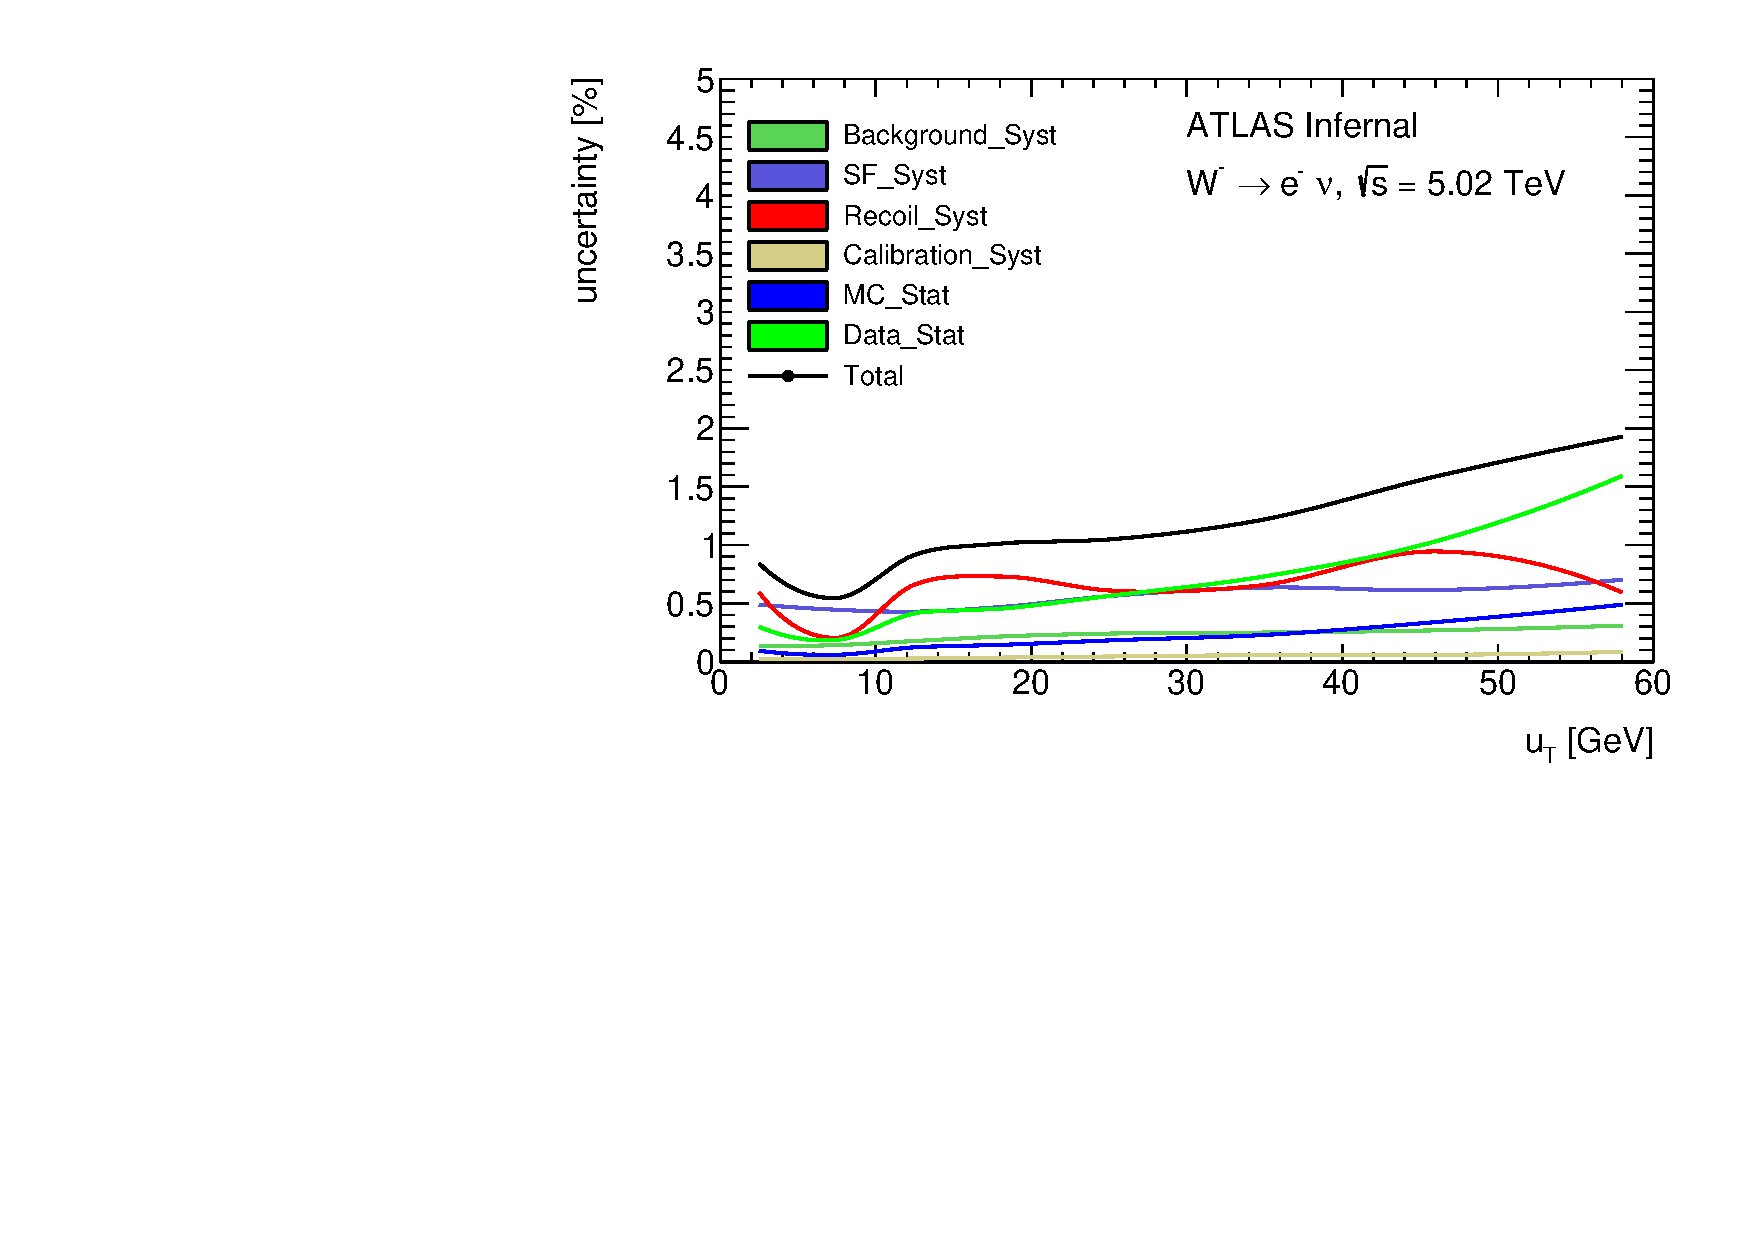
\includegraphics[width=.49\textwidth]{errors_WpT_Reco_cut7_minusenu_5TeV_test1_Unfolded}}
	{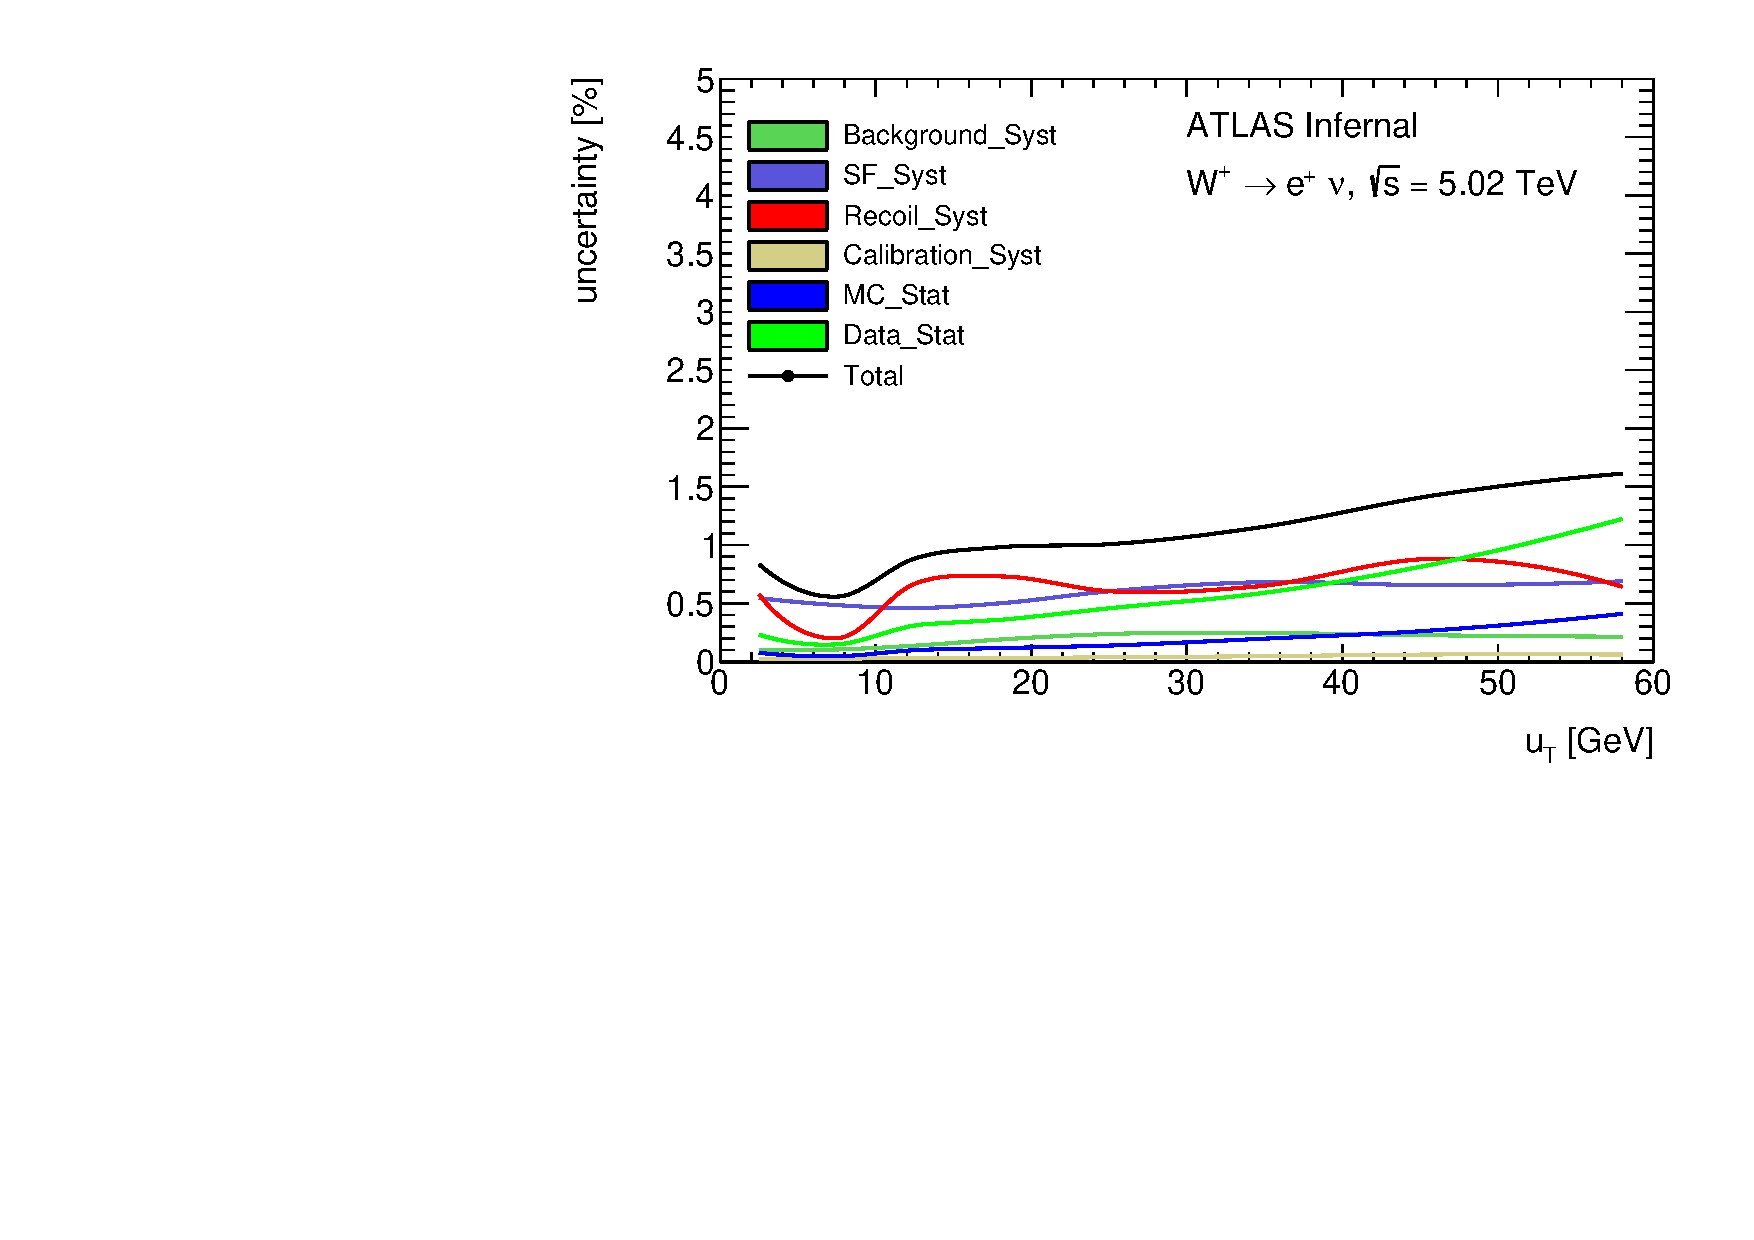
\includegraphics[width=.49\textwidth]{errors_WpT_Reco_cut7_plusenu_5TeV_test1_Unfolded}} \\
	{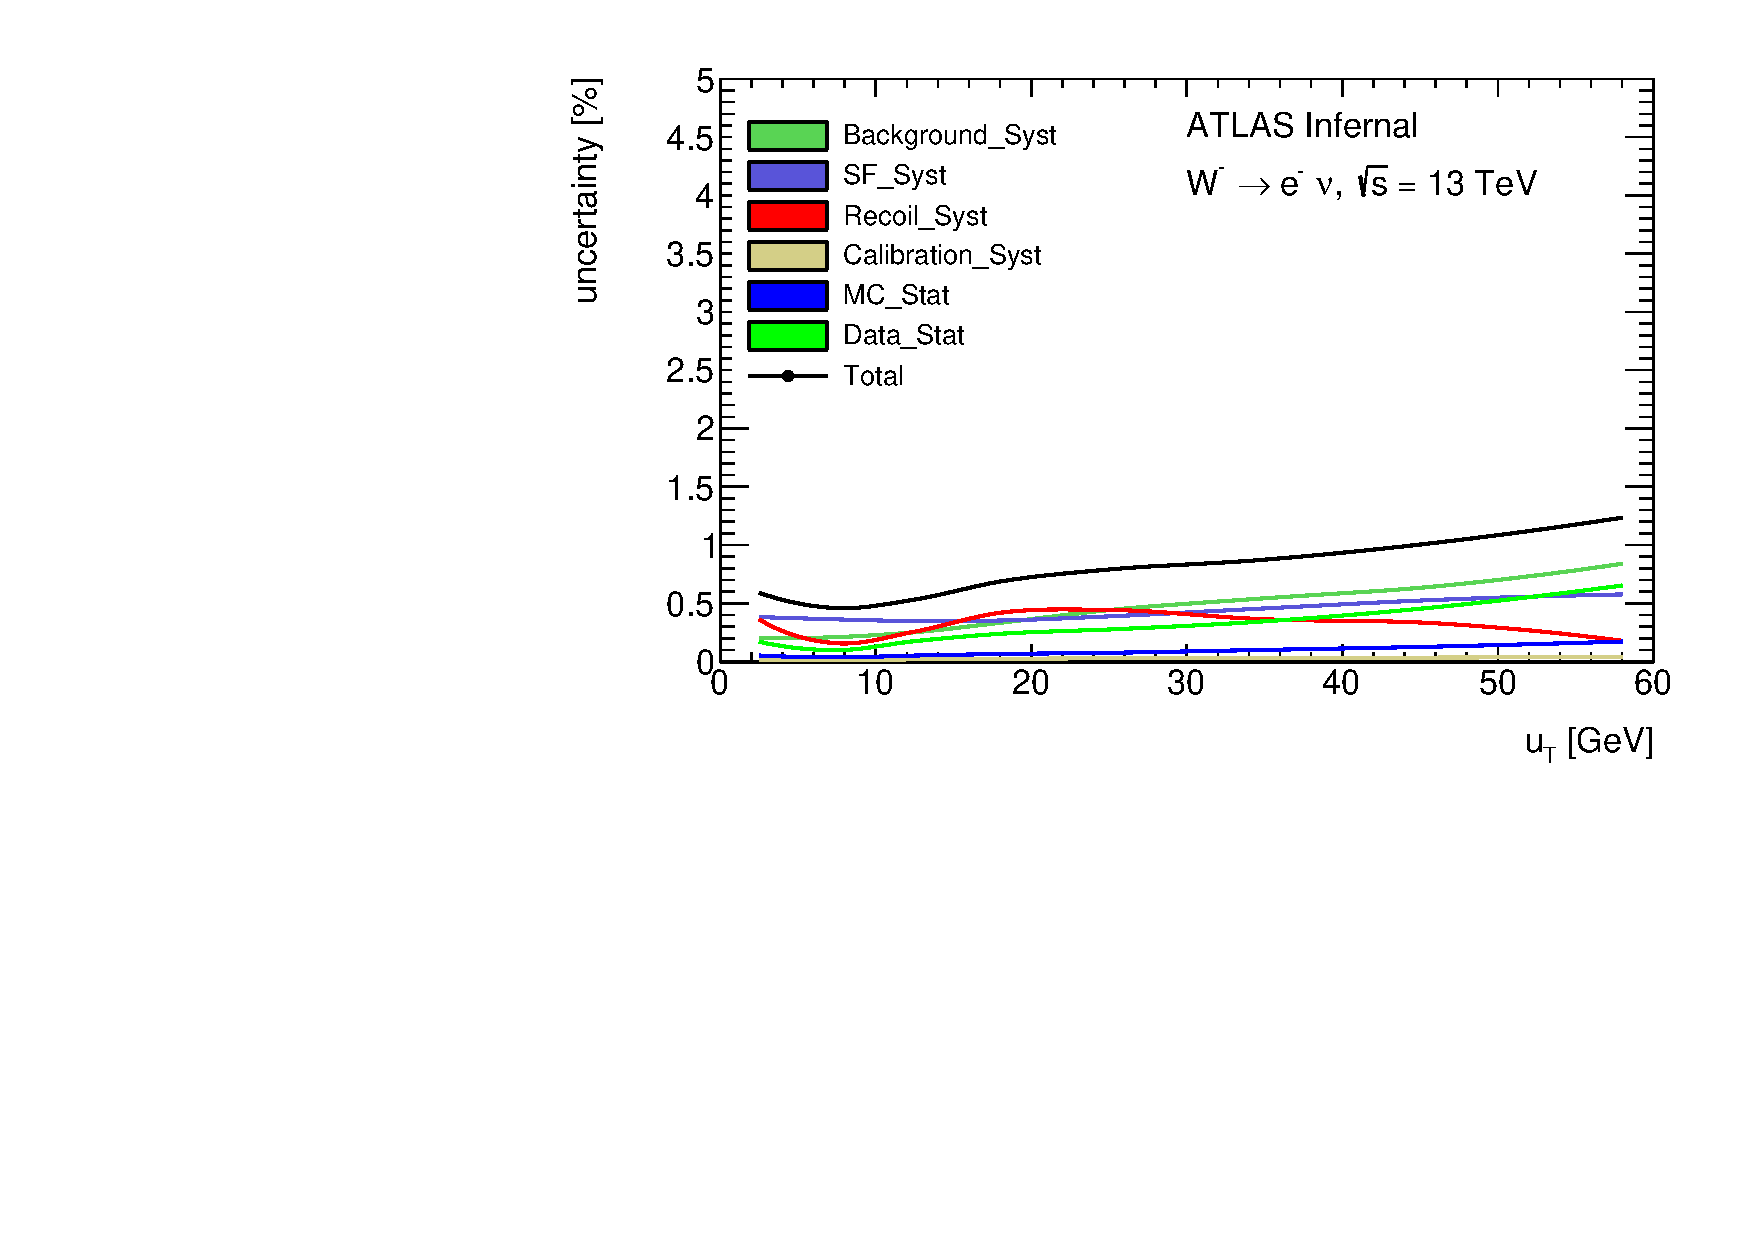
\includegraphics[width=.49\textwidth]{errors_WpT_Reco_cut7_minusenu_13TeV_test1_Unfolded}}
	{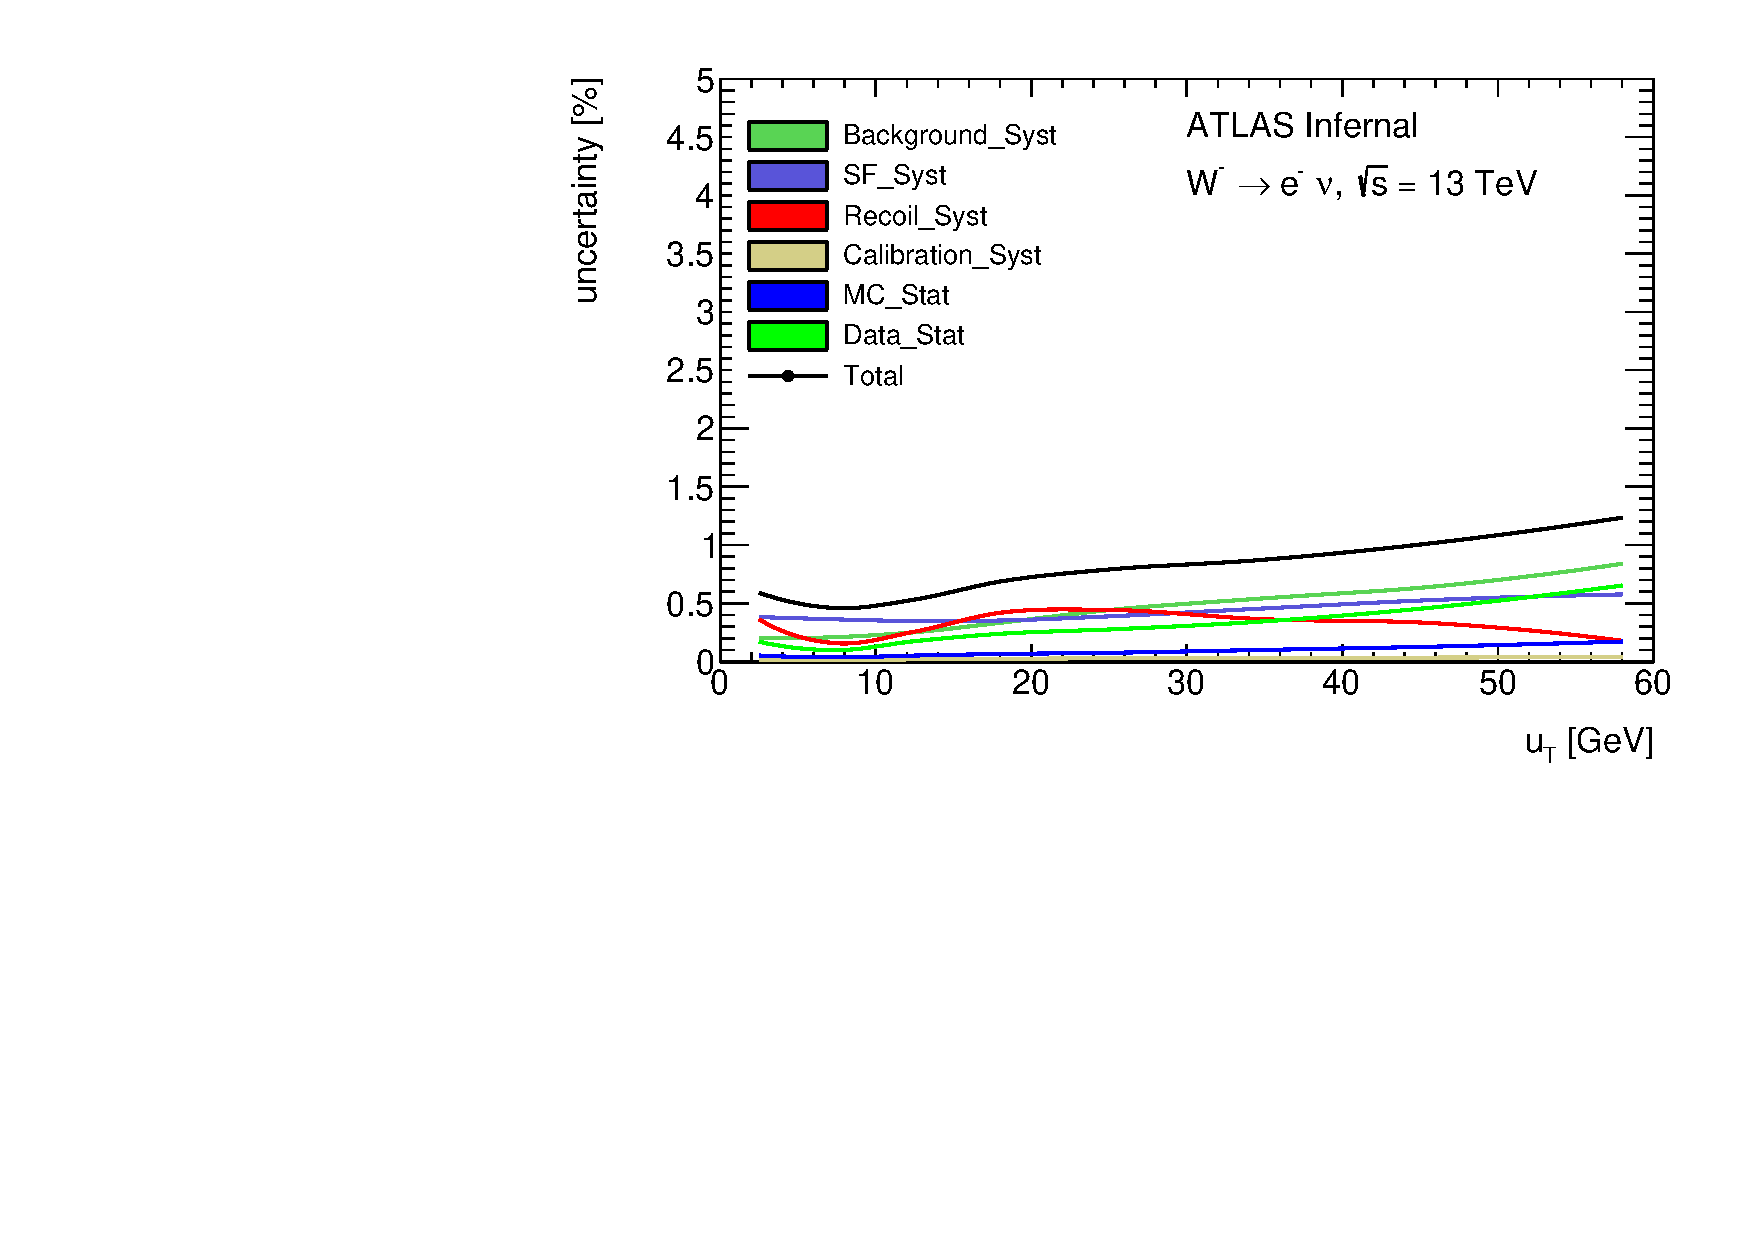
\includegraphics[width=.49\textwidth]{errors_WpT_Reco_cut7_minusenu_13TeV_test1_Unfolded}}
	\caption{ Breakdown of systematic uncertainties for 5 (a,b) and 13 TeV (c,d) in the electron channel at the unfolded level}
	\label{fig:unf_sys_bkd_elec}
\end{figure}

\begin{figure}[h]
	\centering
	{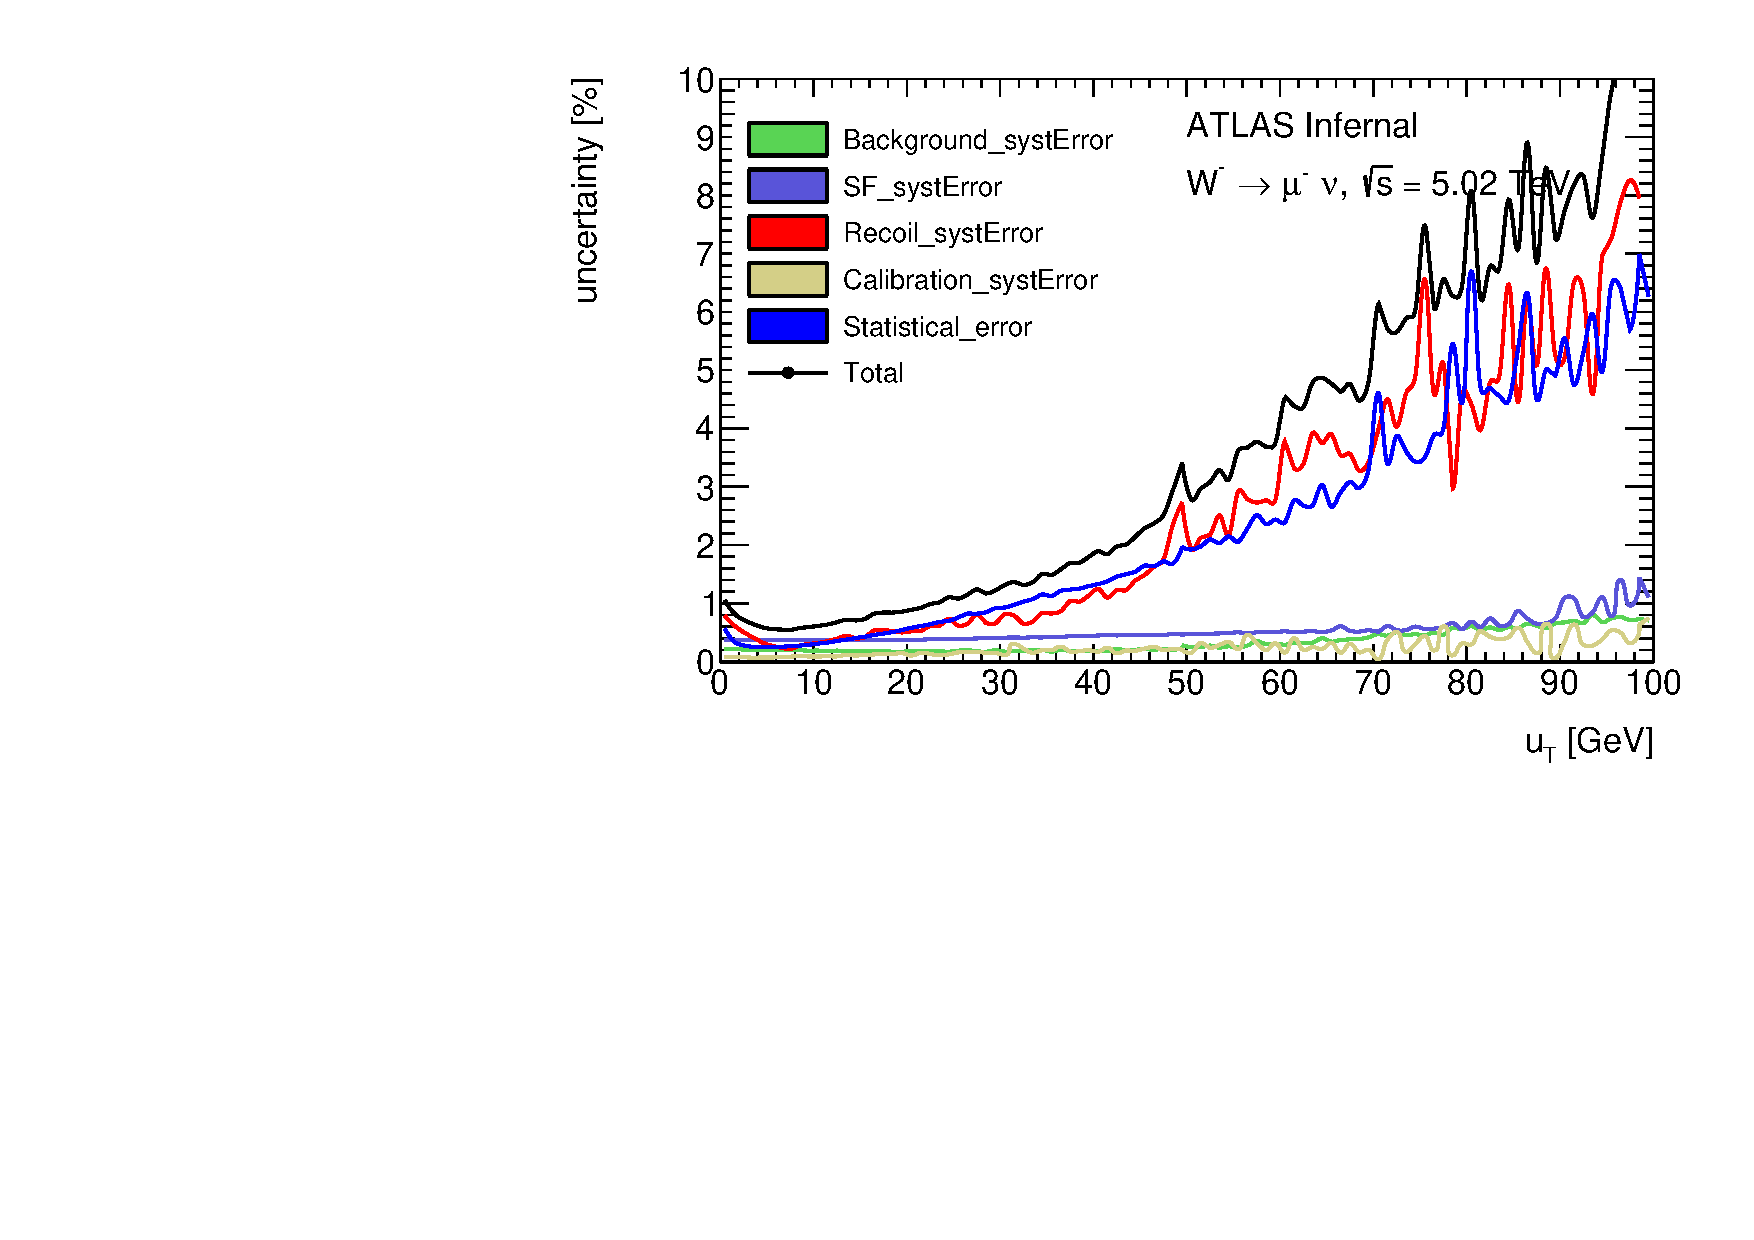
\includegraphics[width=.49\textwidth]{errors_WpT_Reco_cut7_minusmunu_5TeV_test1}}
	{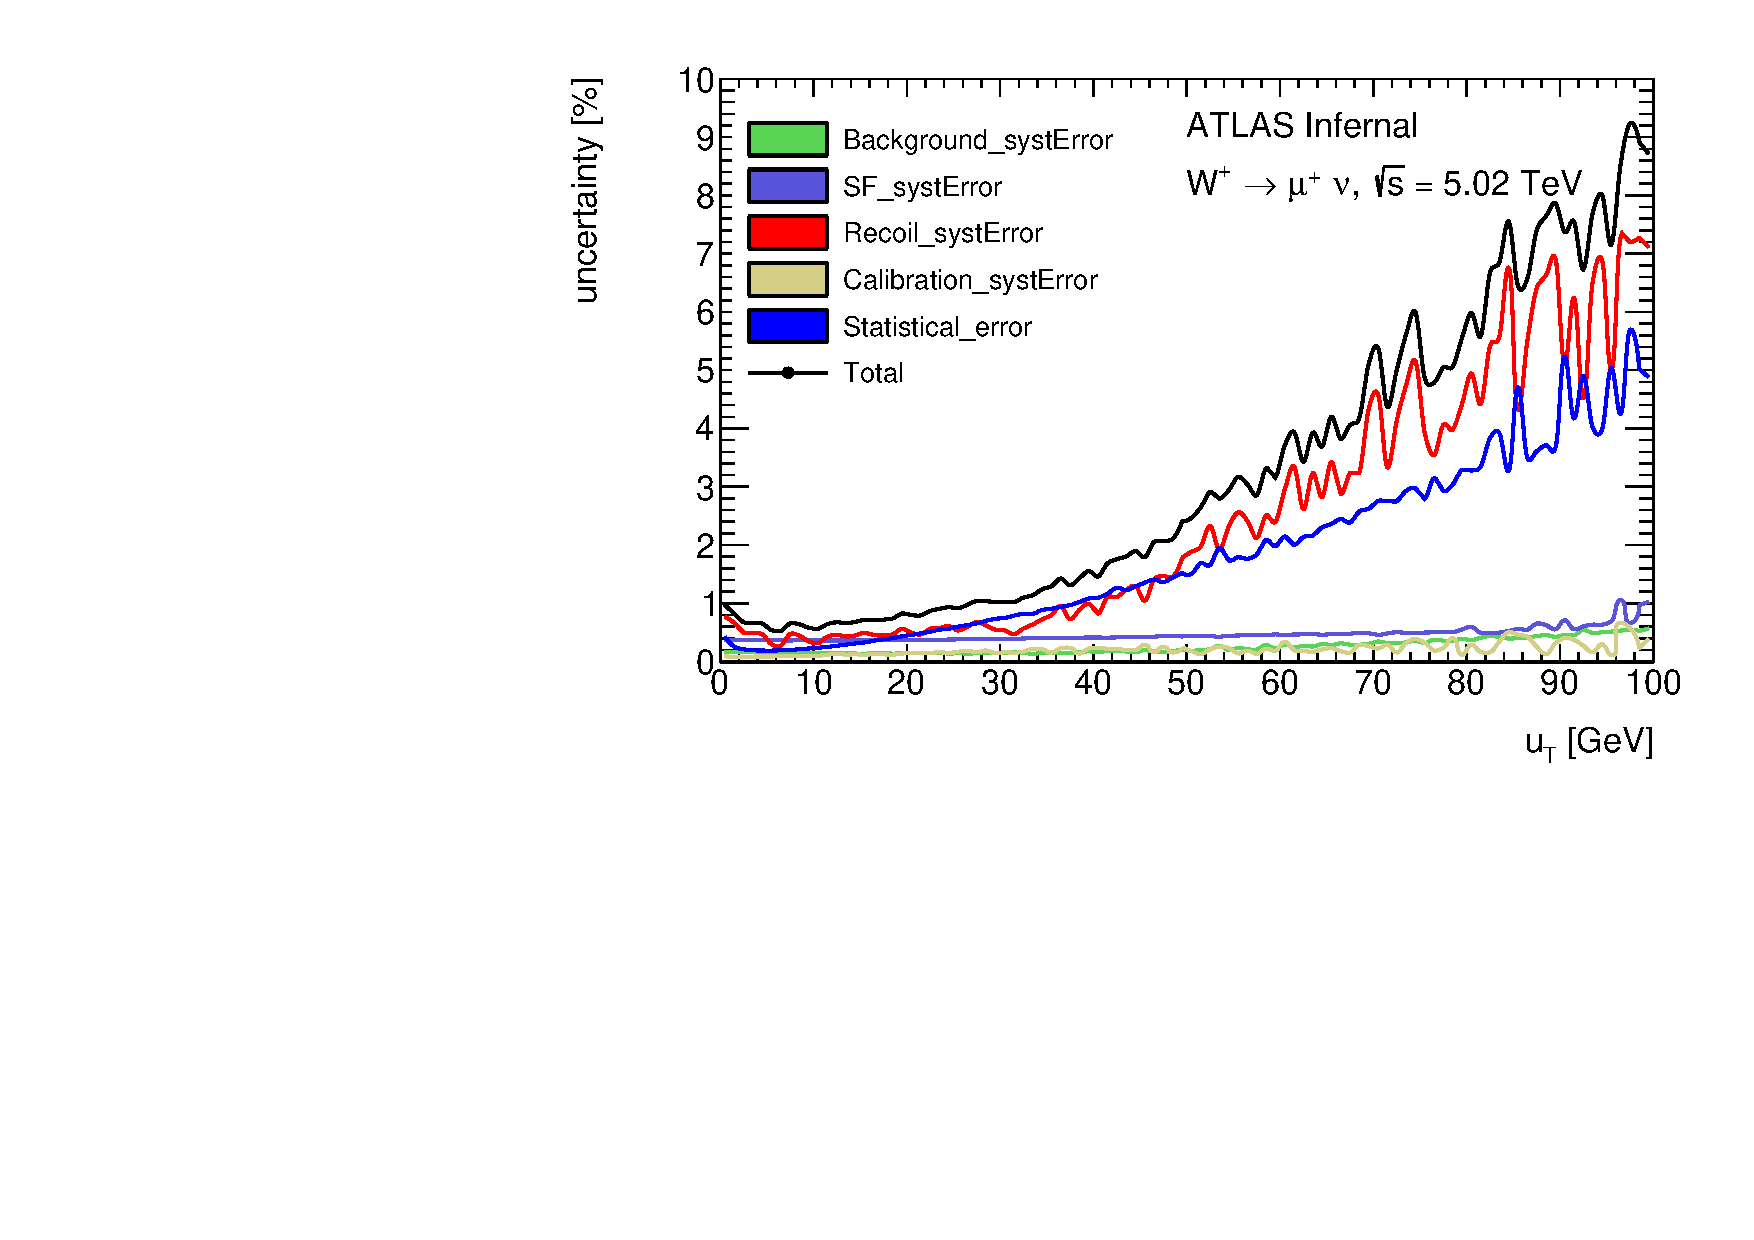
\includegraphics[width=.49\textwidth]{errors_WpT_Reco_cut7_plusmunu_5TeV_test1}} \\
	{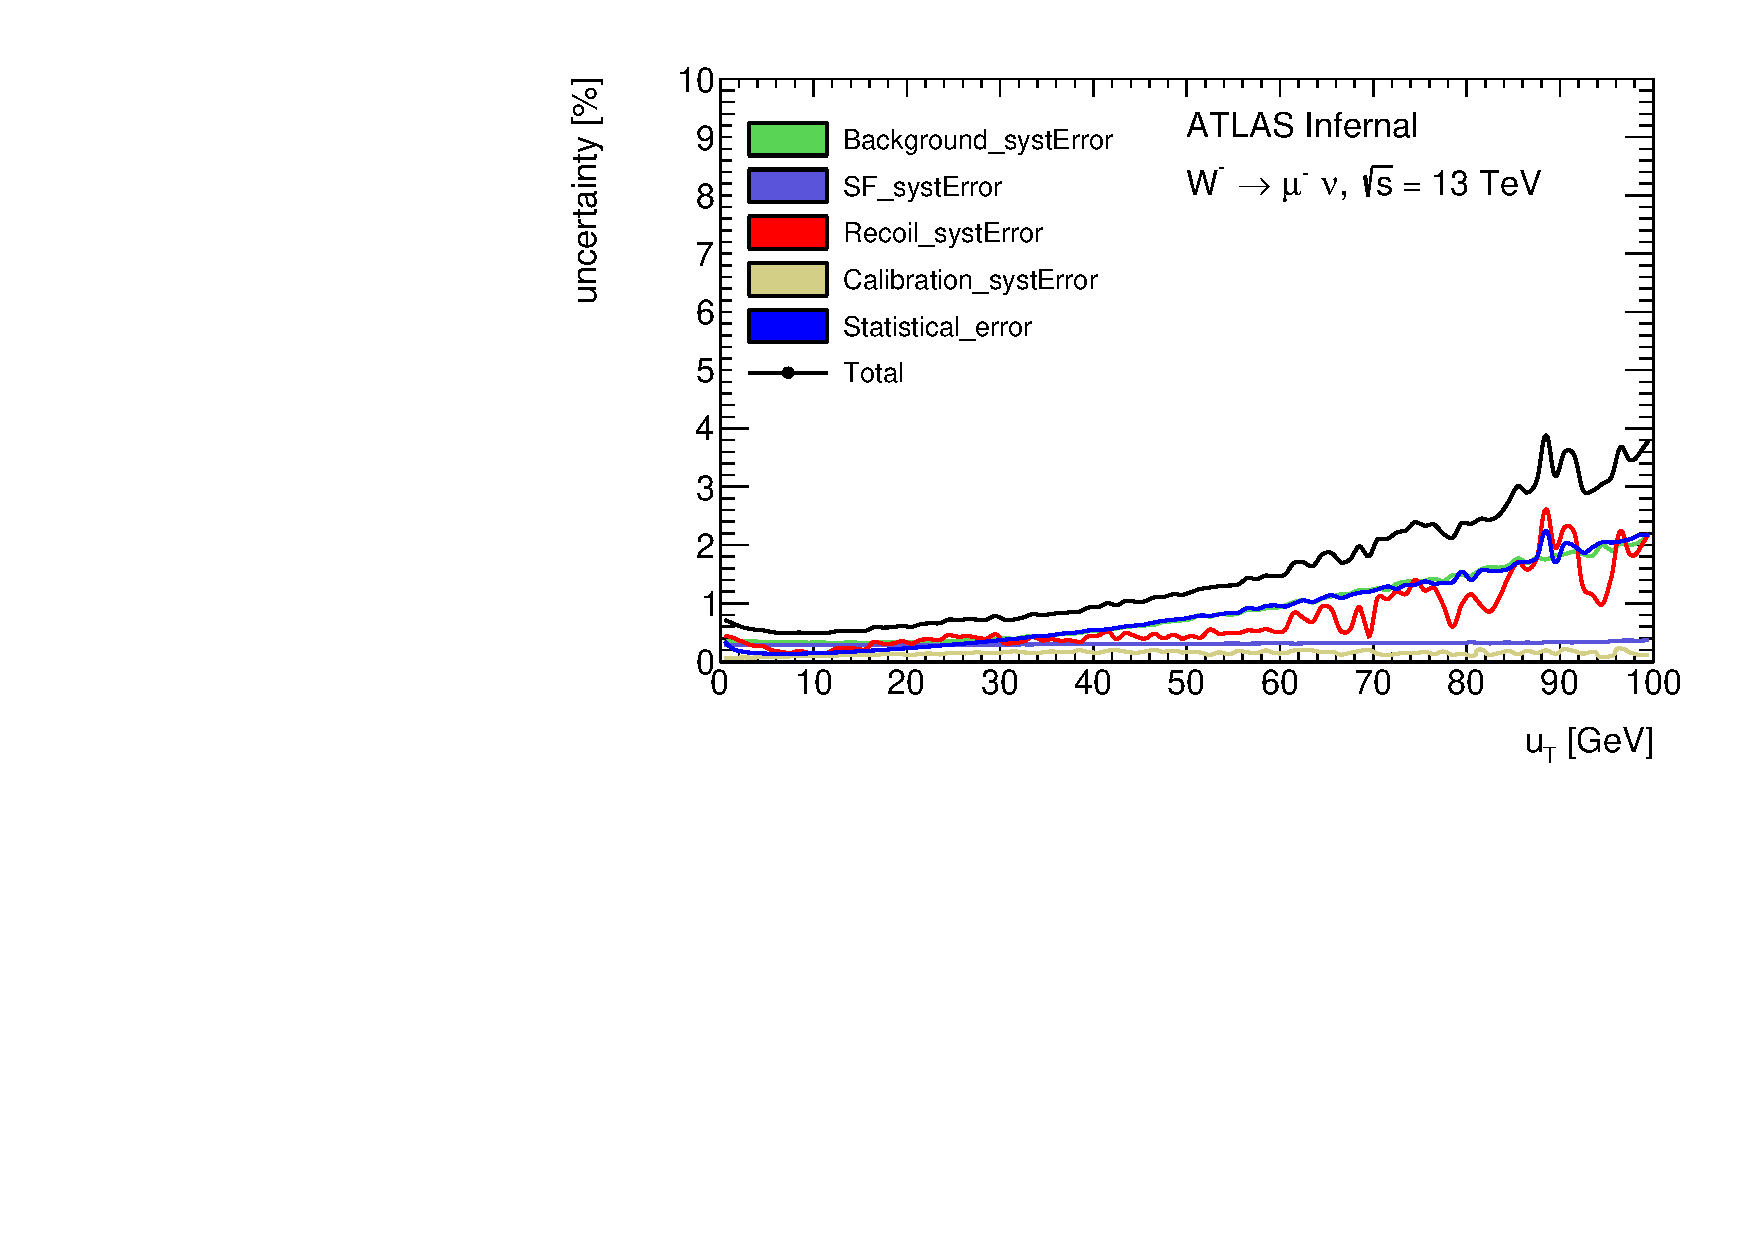
\includegraphics[width=.49\textwidth]{errors_WpT_Reco_cut7_minusmunu_13TeV_test1}}
	{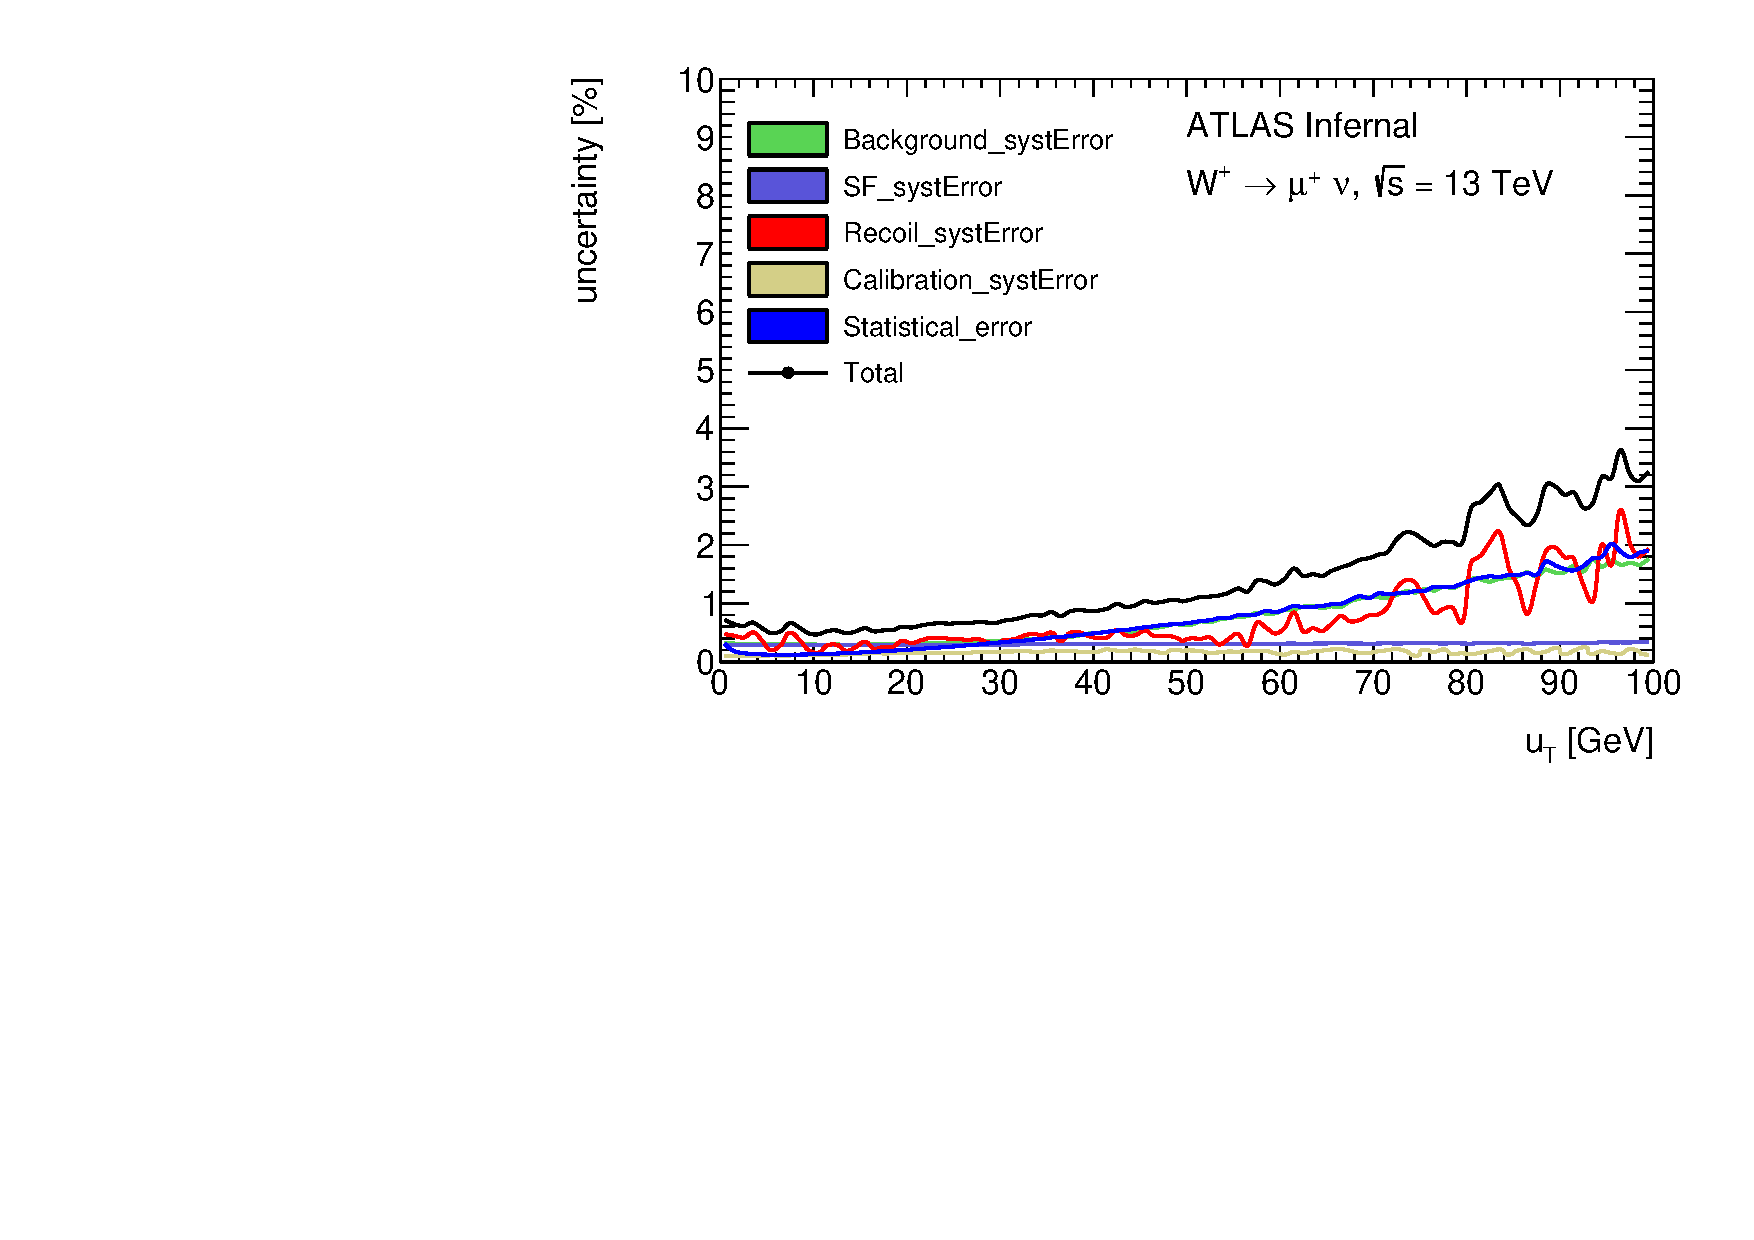
\includegraphics[width=.49\textwidth]{errors_WpT_Reco_cut7_plusmunu_13TeV_test1}}
	\caption{ Breakdown of systematic uncertainties for 5 (a,b) and 13 (c,d) TeV in the muon channel at the reconstructed level}
	\label{fig:reco_sys_bkd_muons}
\end{figure}

\begin{figure}[h]
	\centering
	{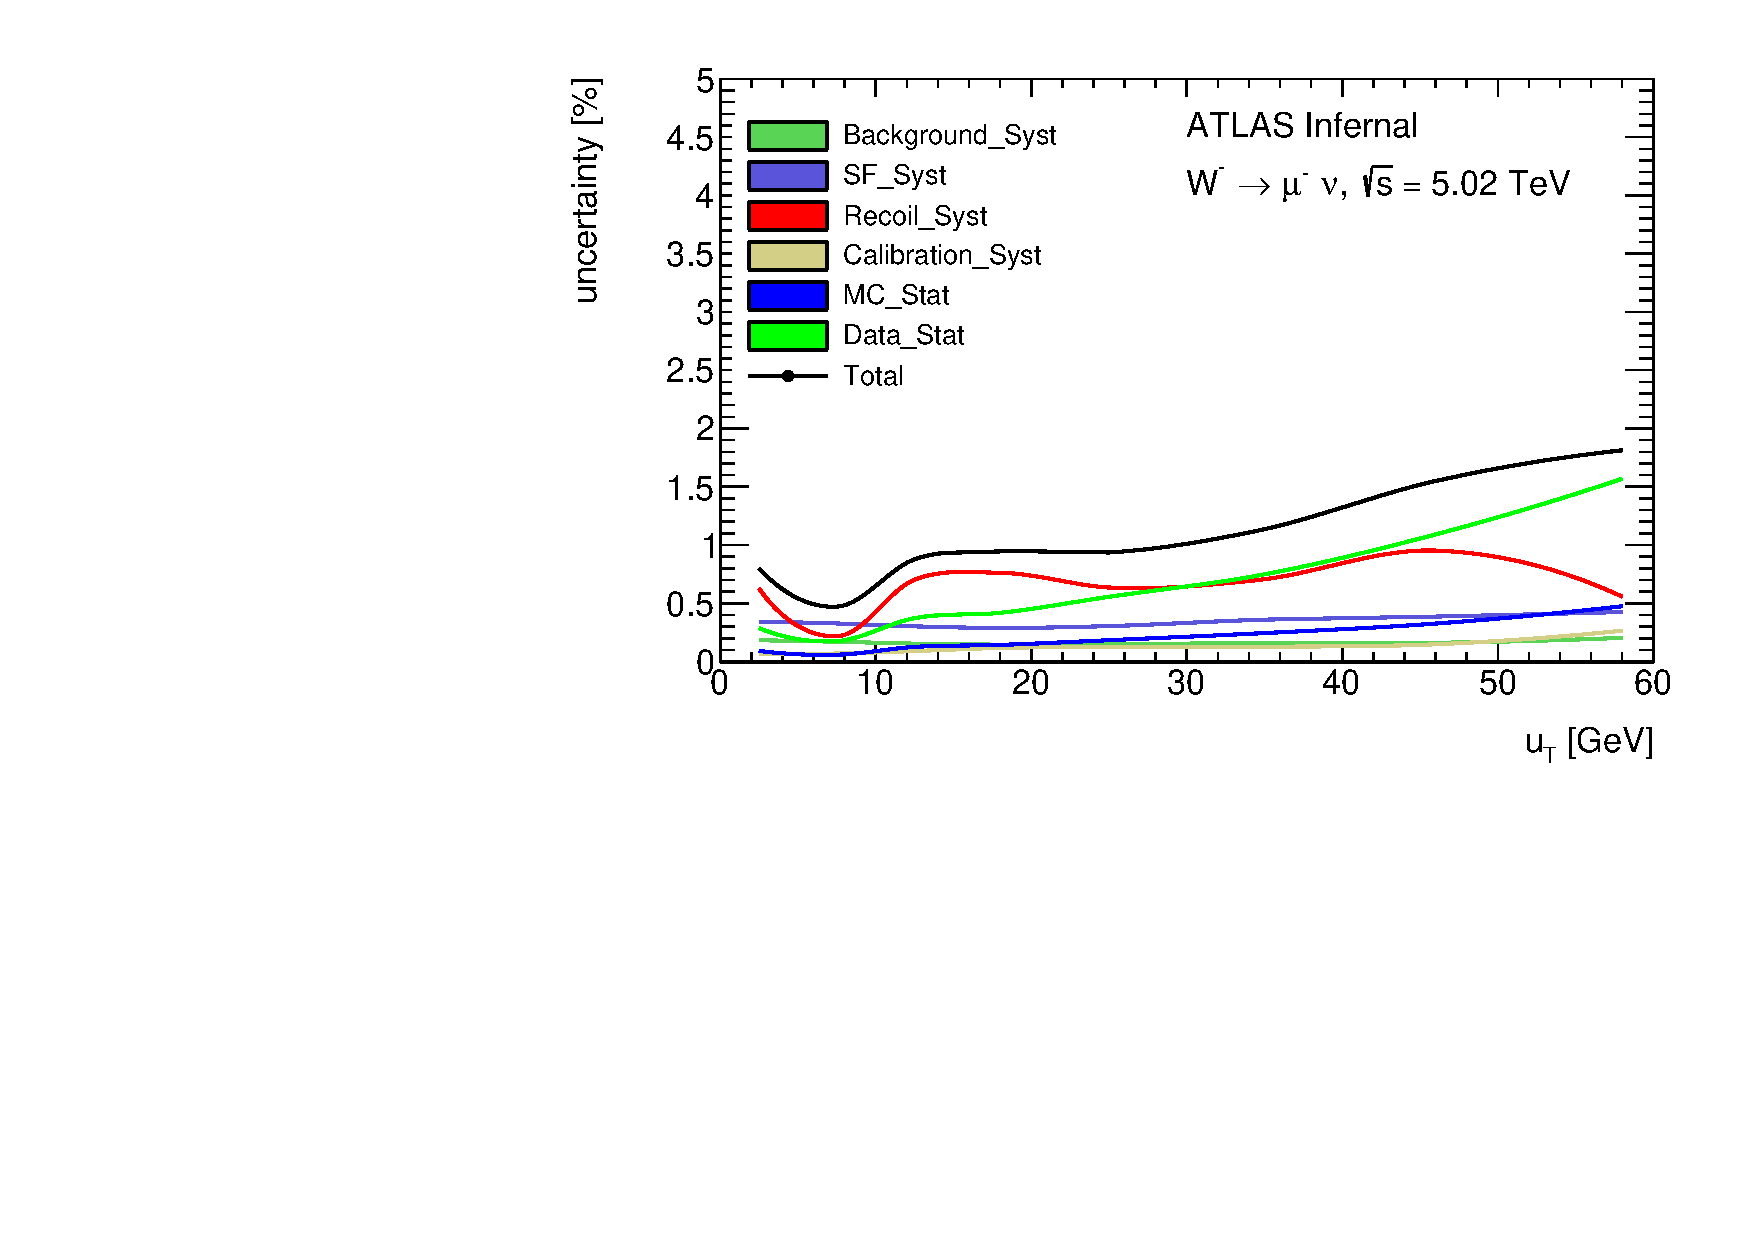
\includegraphics[width=.49\textwidth]{errors_WpT_Reco_cut7_minusmunu_5TeV_test1_Unfolded}}
	{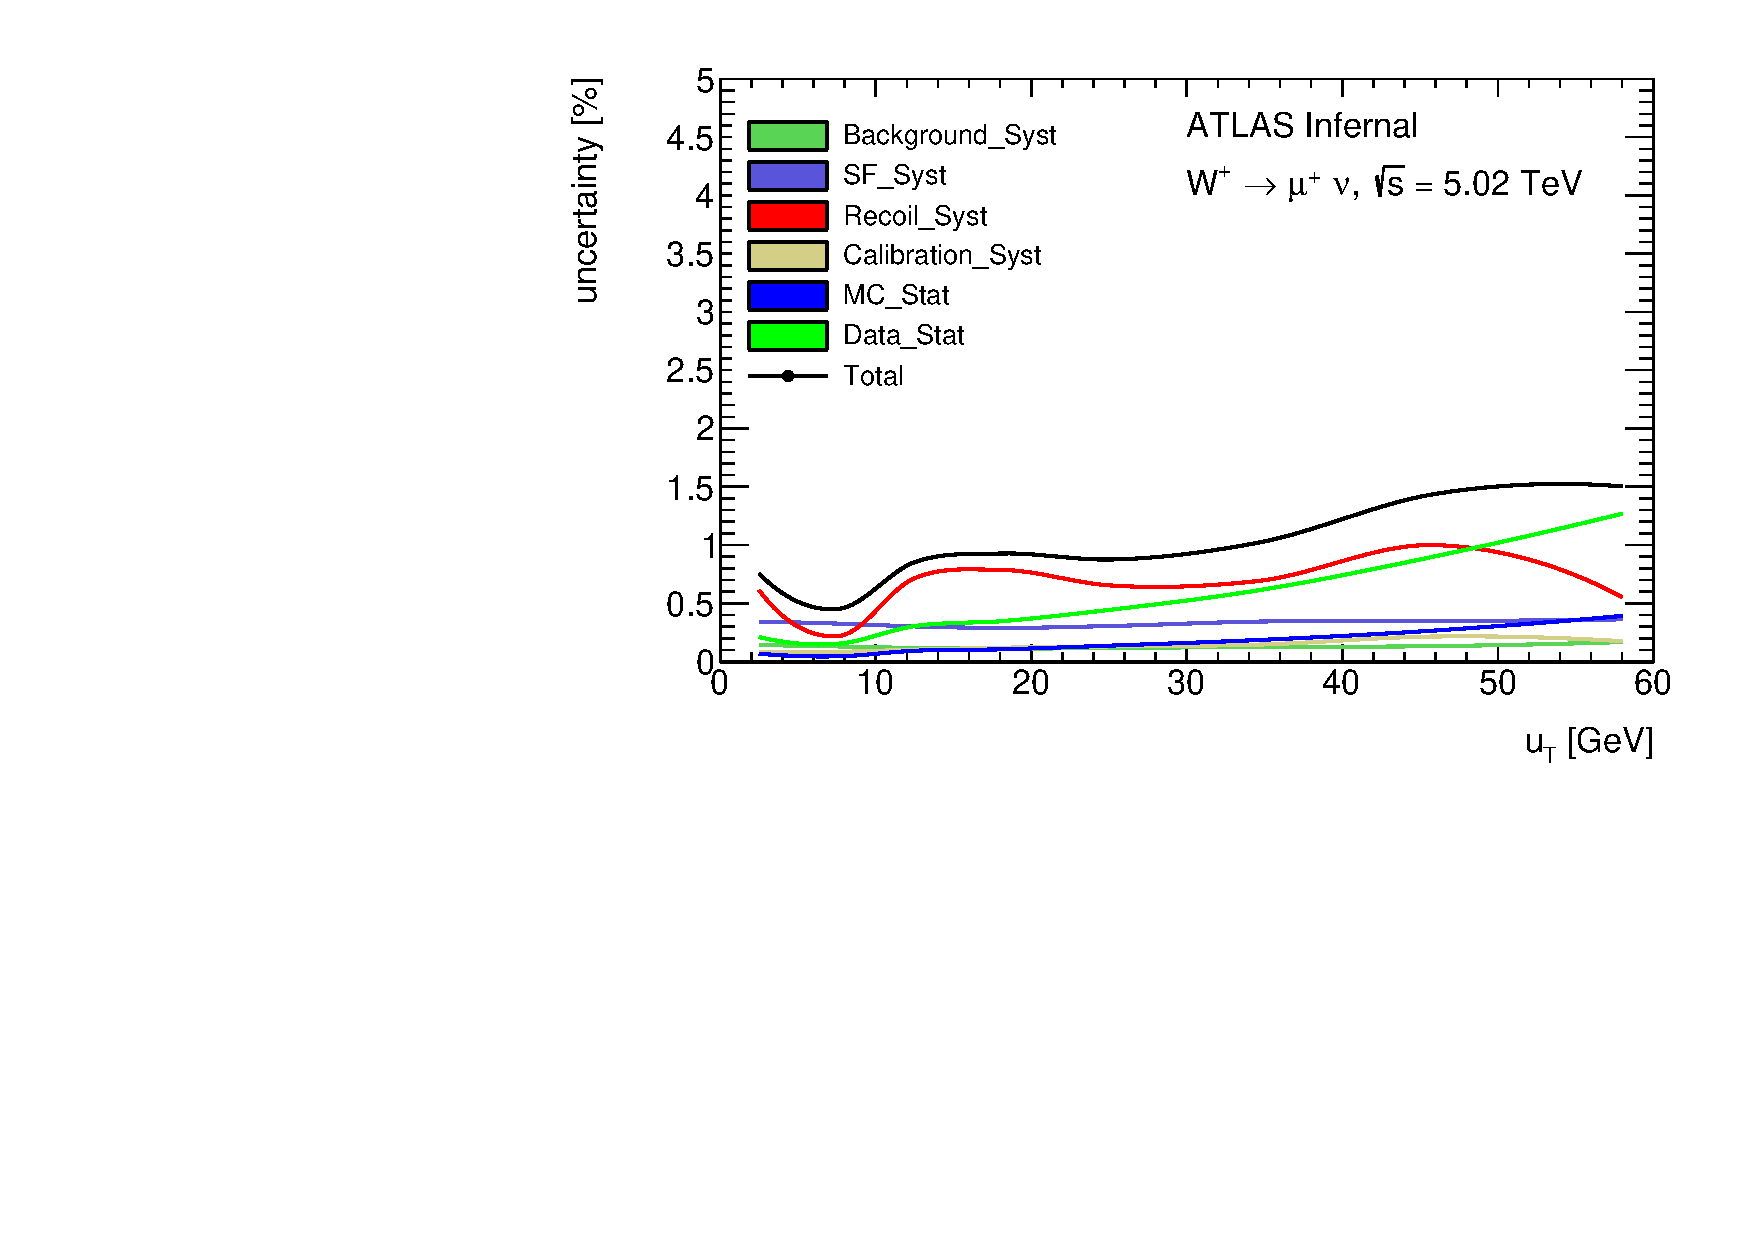
\includegraphics[width=.49\textwidth]{errors_WpT_Reco_cut7_plusmunu_5TeV_test1_Unfolded}} \\
	{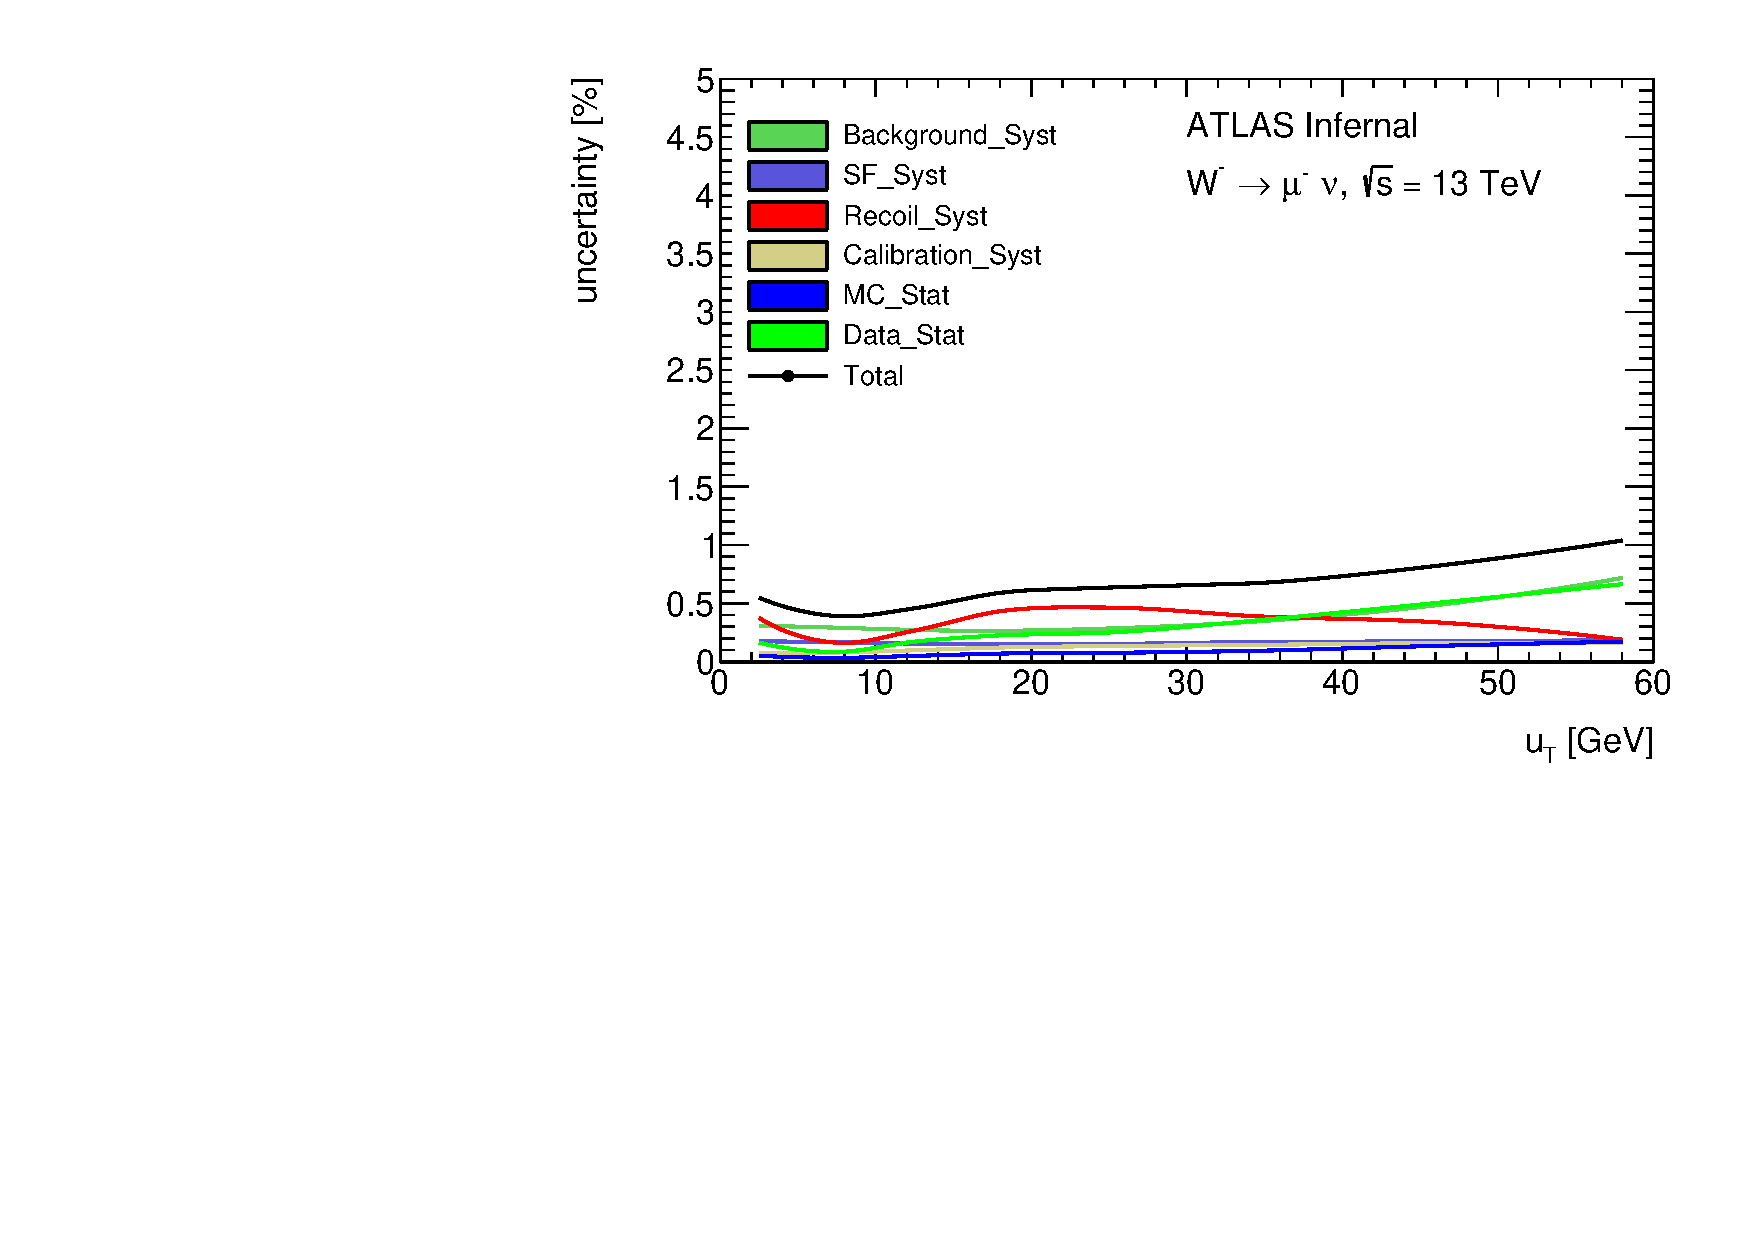
\includegraphics[width=.49\textwidth]{errors_WpT_Reco_cut7_minusmunu_13TeV_test1_Unfolded}}
	{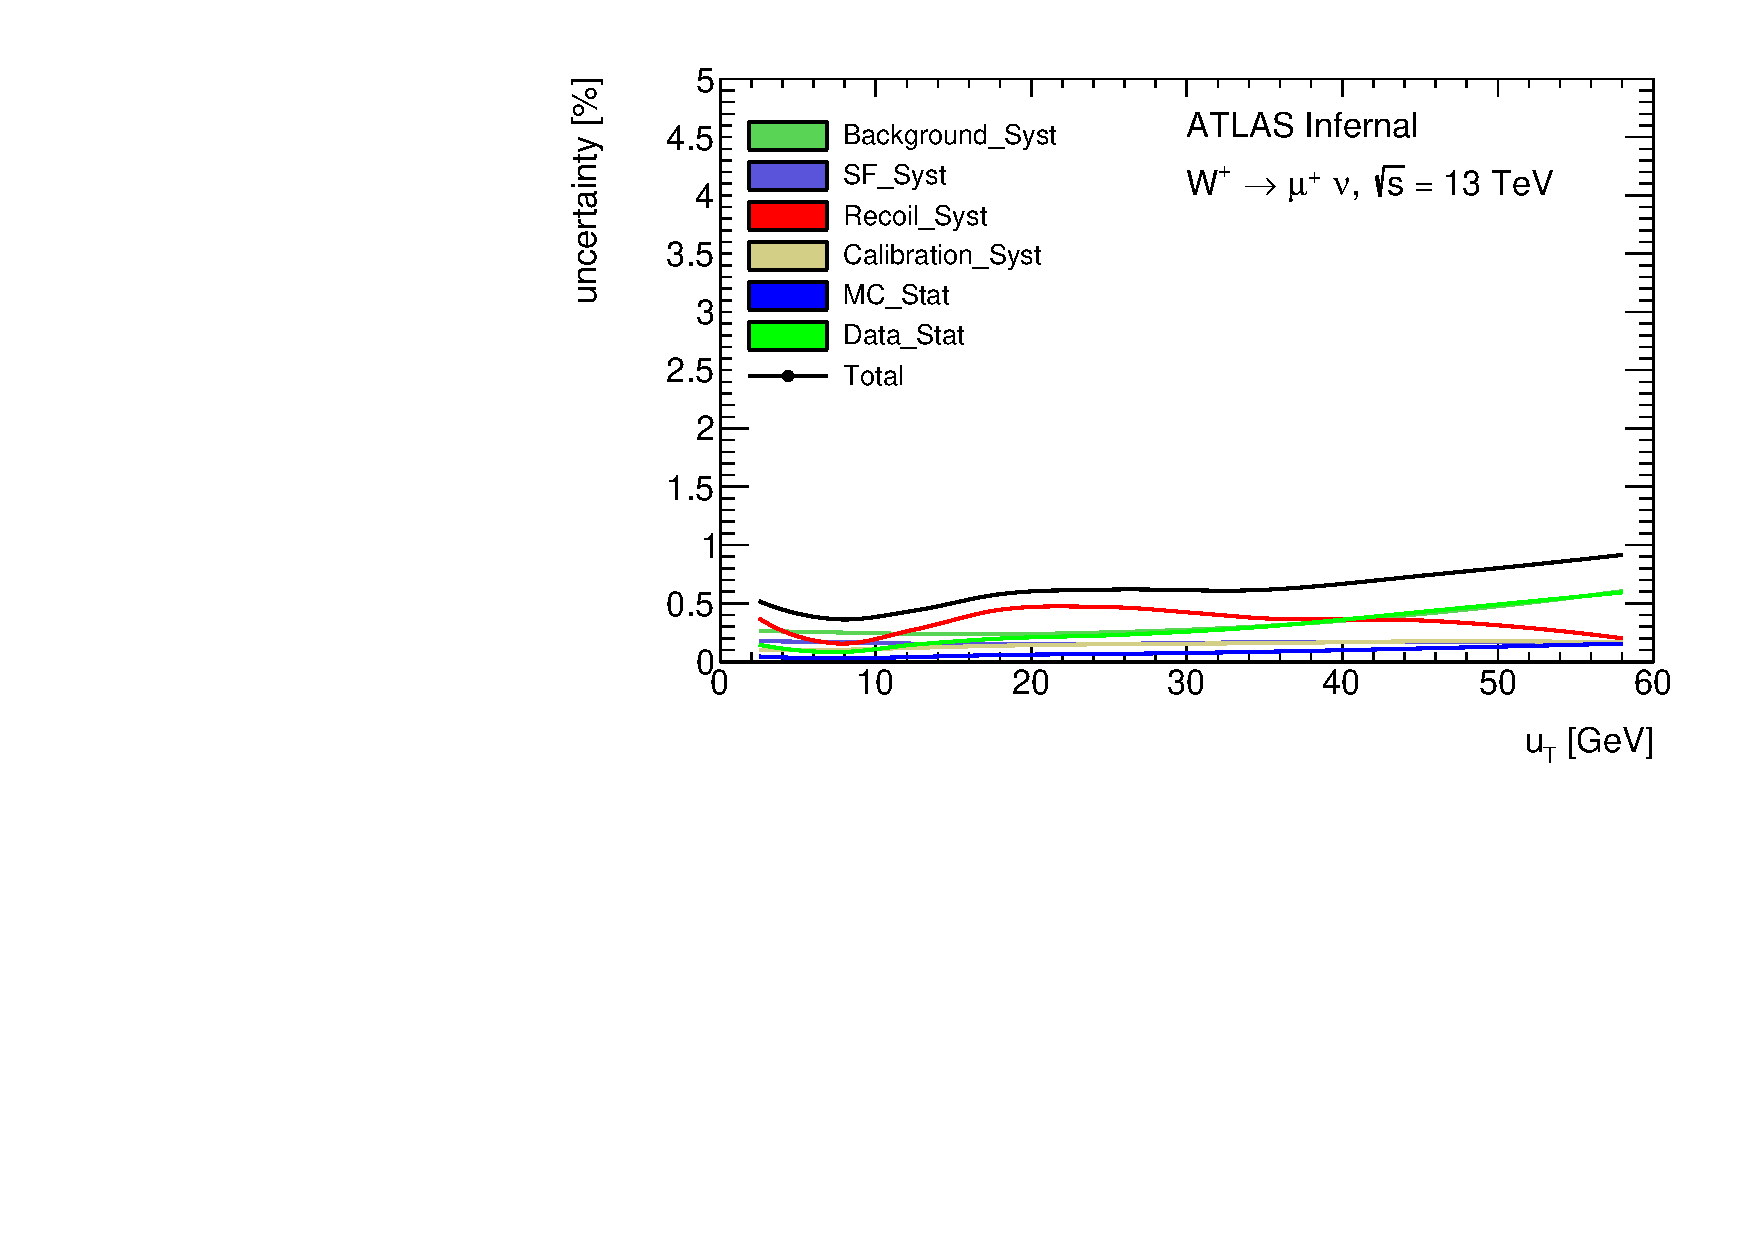
\includegraphics[width=.49\textwidth]{errors_WpT_Reco_cut7_plusmunu_13TeV_test1_Unfolded}}
	\caption{ Breakdown of systematic uncertainties for 5 (a,b) and 13 TeV (c,d) in the muon channel at the unfolded level}
	\label{fig:unf_sys_bkd_muons}
\end{figure}
\clearpage
\section{Unfolding bias}
One of the uncertainties associated with unfolding usage is called unfolding bias and may arise because the procedure relies on the MC simulation of the distribution, which is used as a prior hypothesis for the Bayesian algorithm. Possible discrepancies between the modelled and true distribution lead to erroneous  bin-to-bin migrations and can lead to distortions of the spectrum.\\
In order to estimate the bias induced by the unfolding procedure it is necessary to quantify how much the unfolded result is impacted by the assumed MC distribution. A set of samples with a different distribution at the truth level though compatible at the detector level is generated. \\

The truth distribution is reweighted until a good agreement between the data and MC is reached at the reconstruction level. The agreement is estimated in the kinematic region of $u_T<100\gev$ using the $\chi^2$ criterion. The truth reweighting procedure is applied to MC samples with a different distribution: \Pythia, Sherpa and DYRES were used. Fig. demonstrates the initial difference in the distributions.\\

The results are presented on fig~\ref{fig:BiasResultLargeBins} for 5~GeV bins and 3 unfolding iterations. The obtained bias is close to the precision goal of the measurement ($\sim~1\%$) for the 5~\TeV dataset. The 13~\TeV\ dataset shows a larger bias, which can be explained by a larger discrepancy between data and Monte-Carlo. Worse resolution in 13~\TeV\ suggests a neccesity to try a broader binning comparing to 5~\GeV.

\begin{figure}[h]
	\centering
	{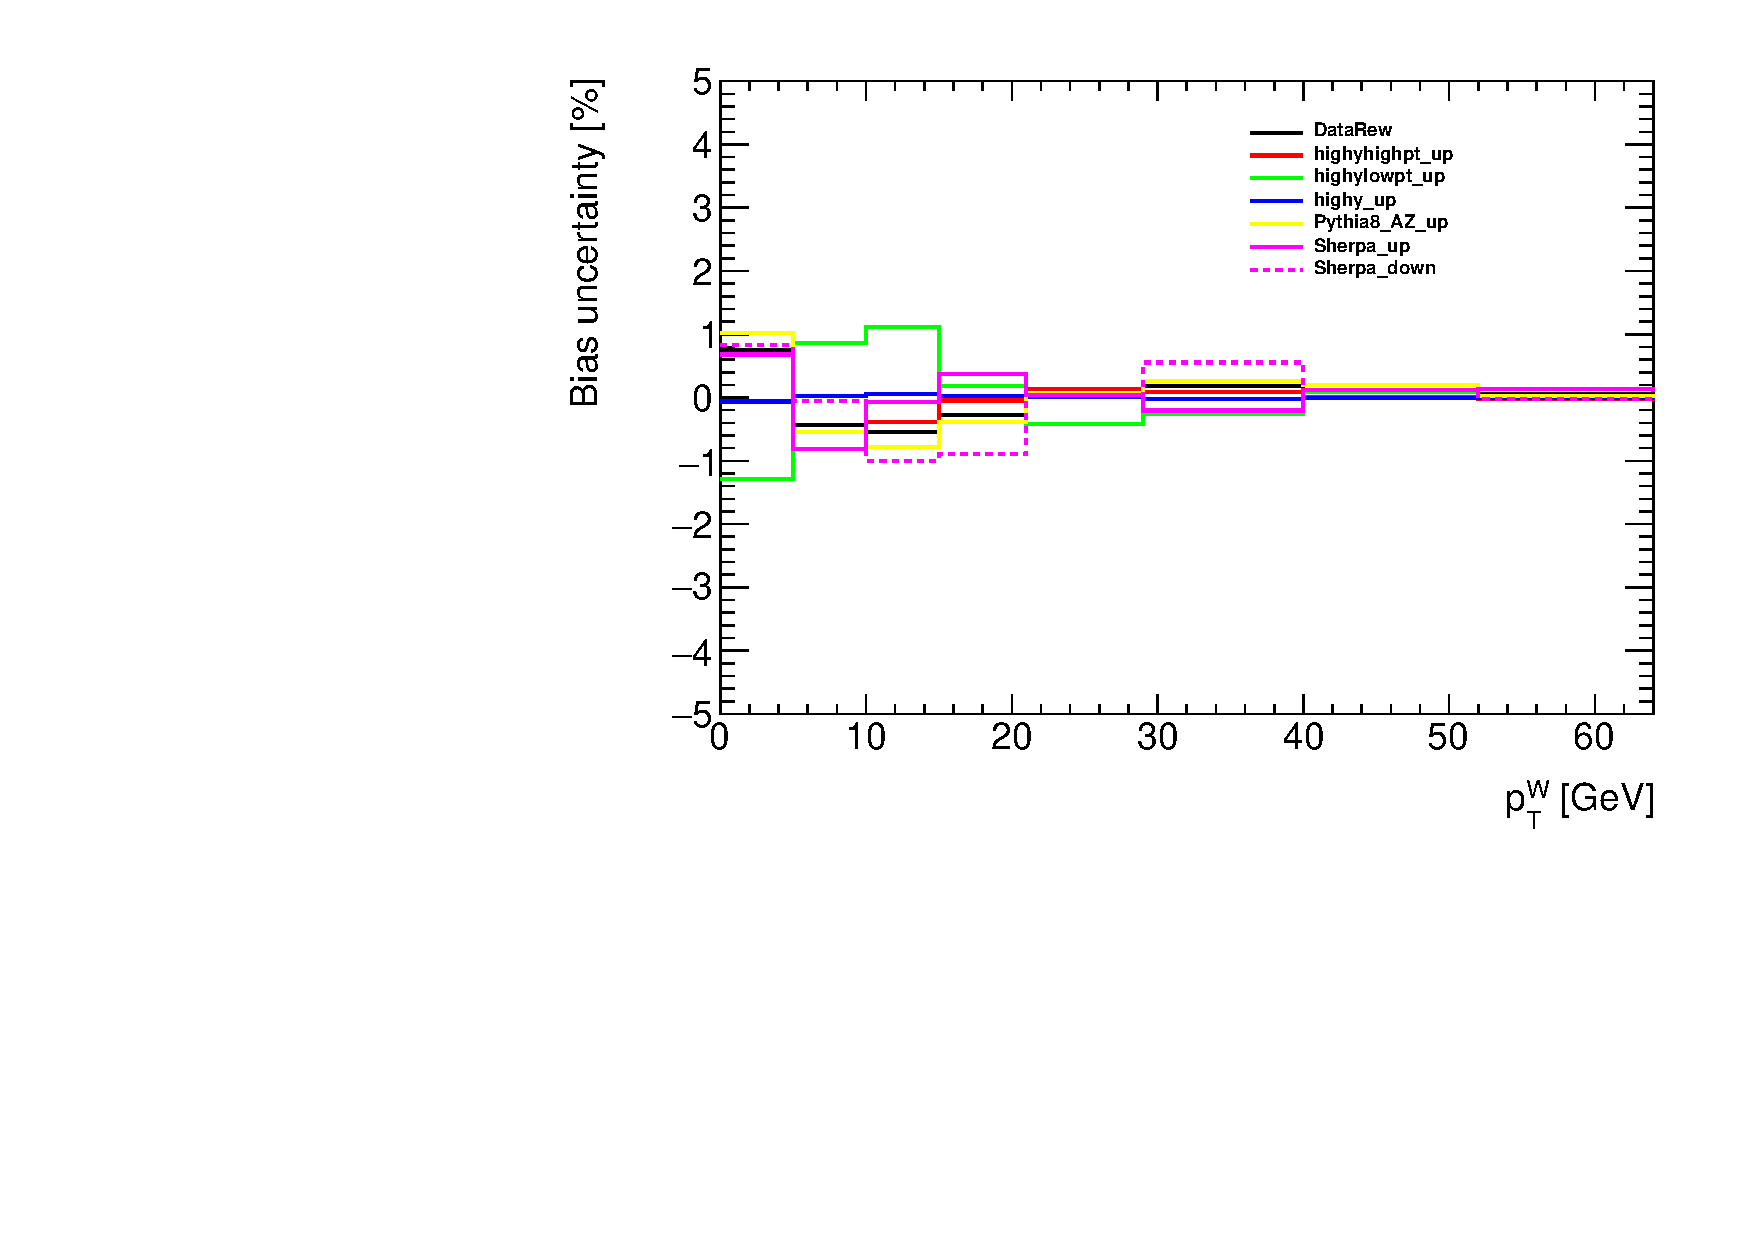
\includegraphics[width=.49\textwidth]{bias_sqrts5_iter3_Wminusenu_fileJan_largebins.pdf}}
	{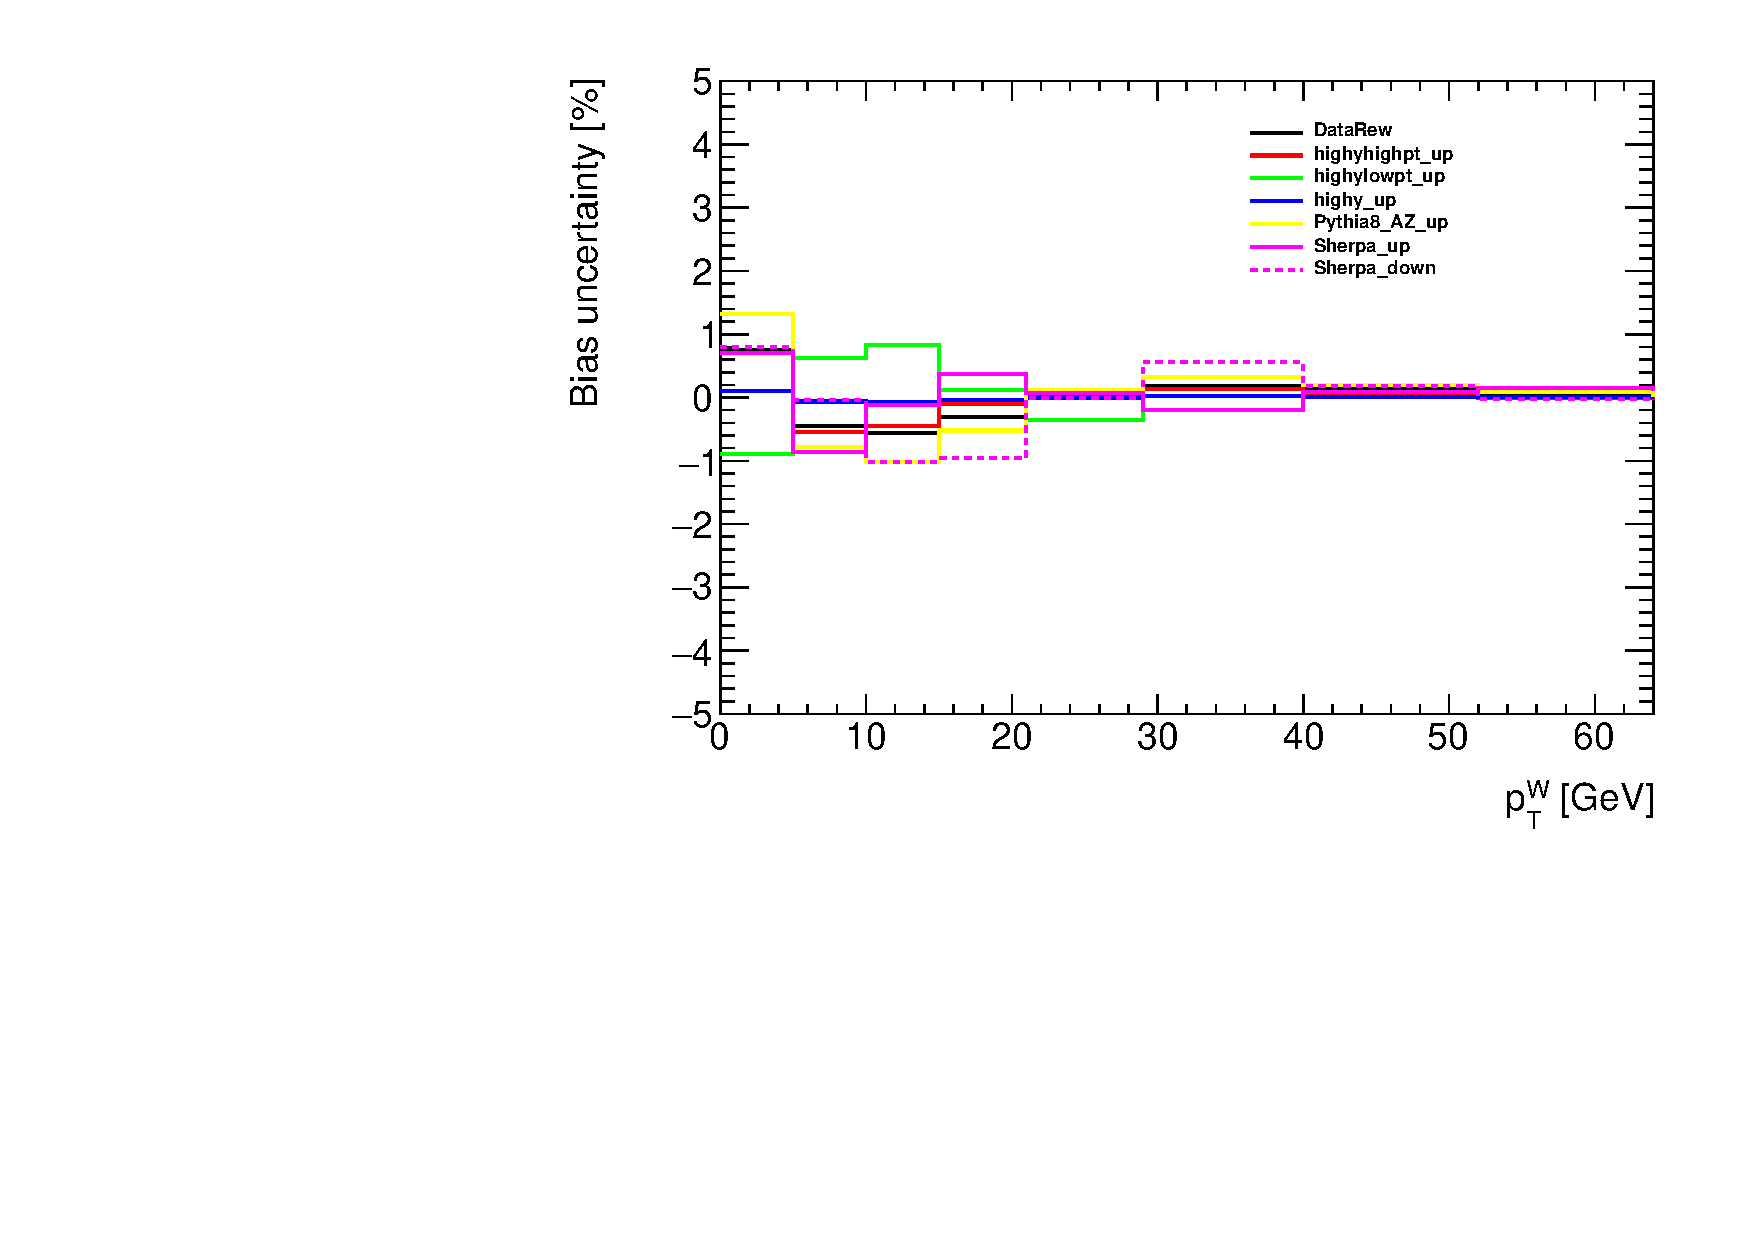
\includegraphics[width=.49\textwidth]{bias_sqrts5_iter3_Wplusenu_fileJan_largebins.pdf}}\\
	{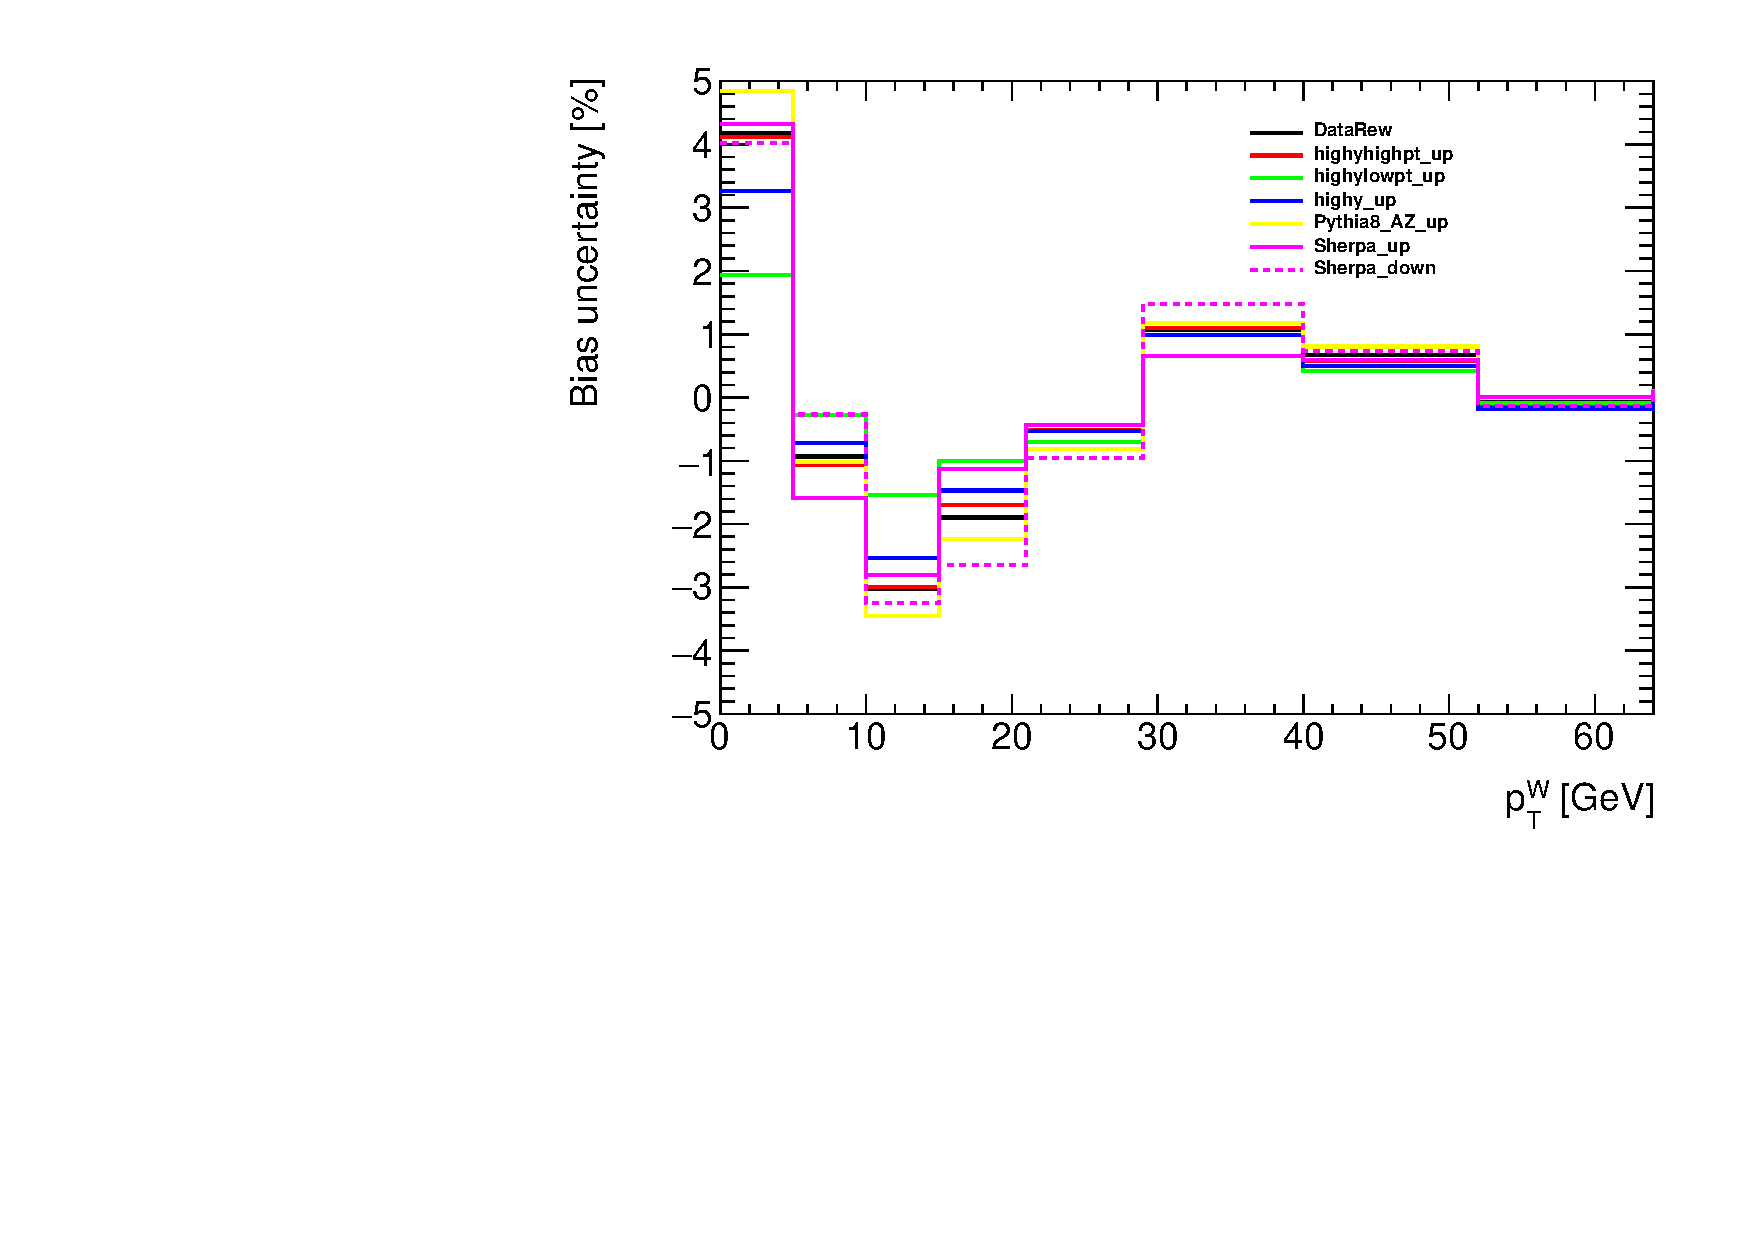
\includegraphics[width=.49\textwidth]{bias_sqrts13_iter3_Wminusenu_fileJan_largebins.pdf}}
	{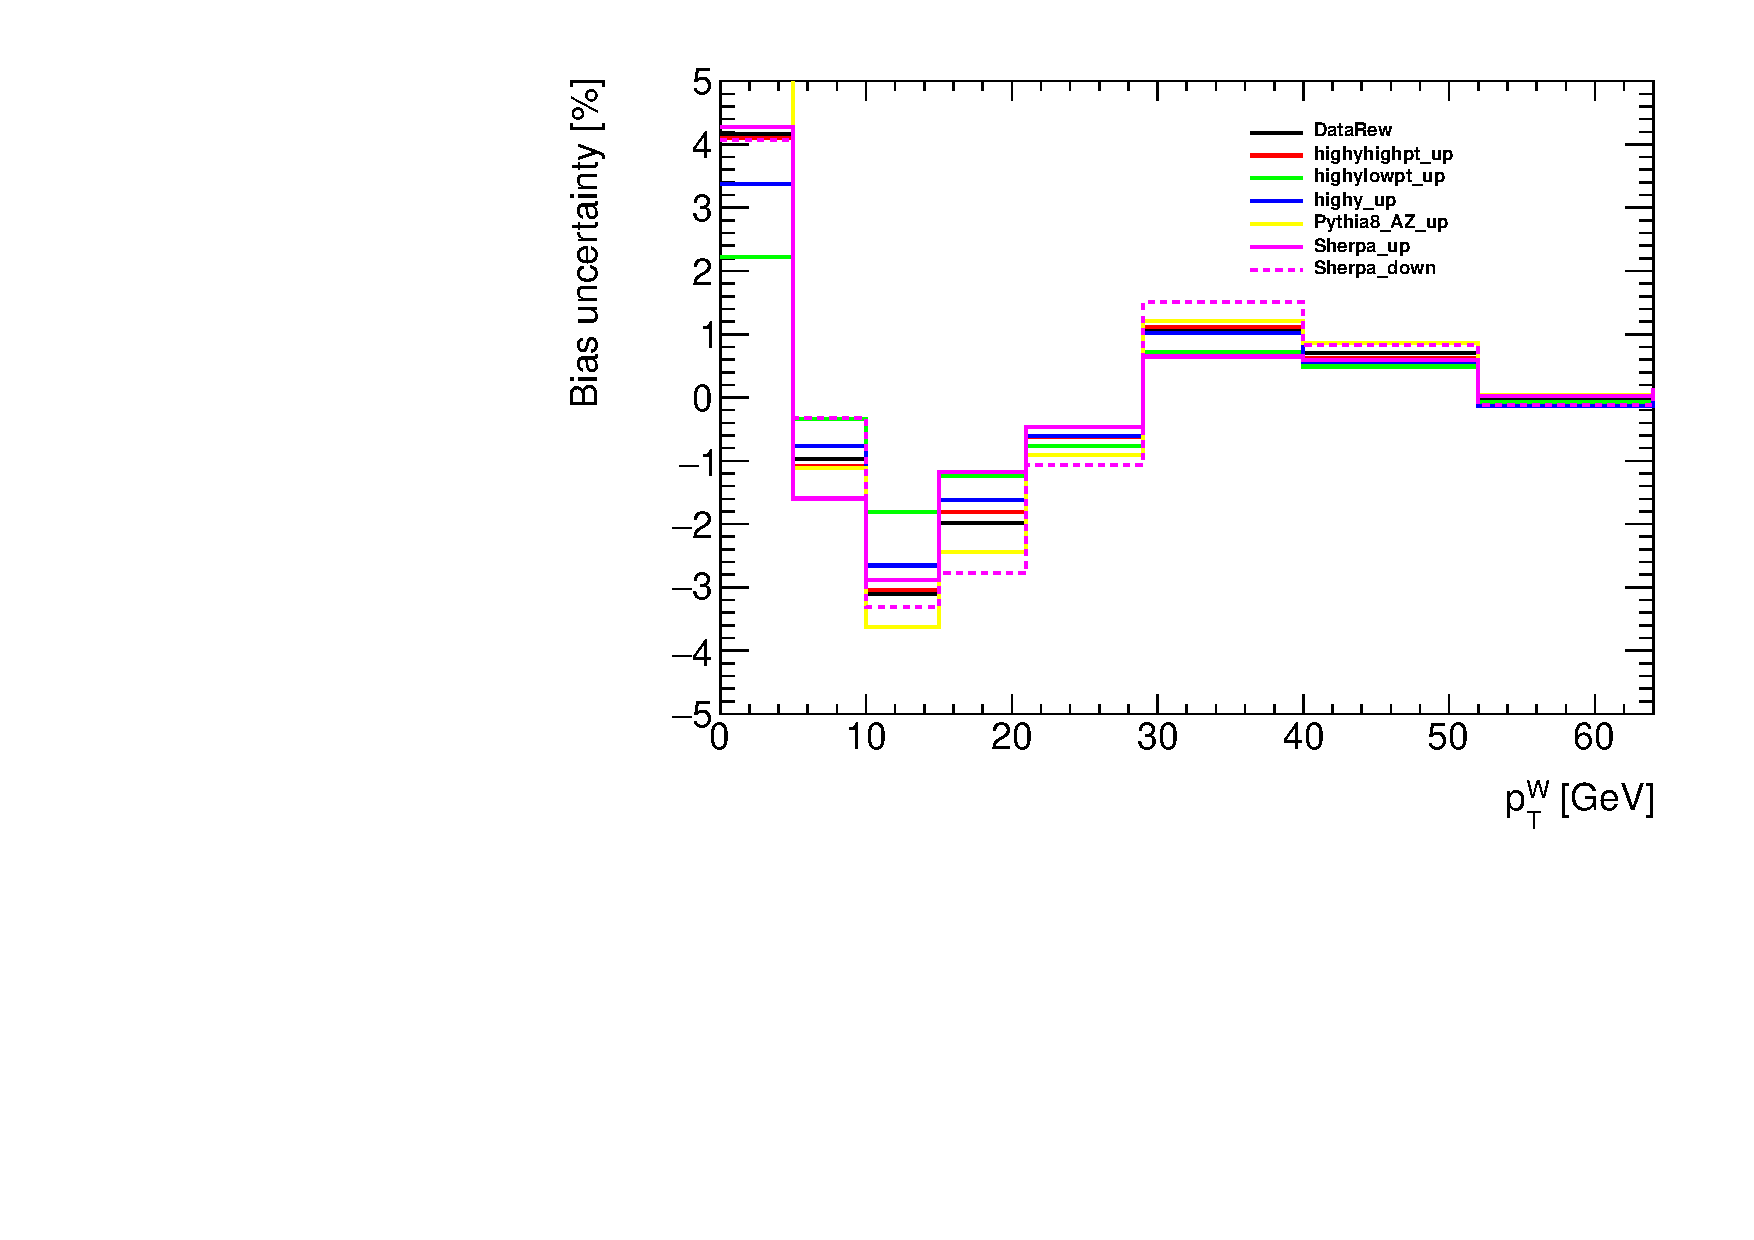
\includegraphics[width=.49\textwidth]{bias_sqrts13_iter3_Wplusenu_fileJan_largebins.pdf}}
	\caption{Unfolding bias on \ptw\ in the electron channel after 3 iterations, for $W^-$ (left) and $W^+$ (right), at 5~TeV (top) and 13~TeV (bottom).}
	\label{fig:BiasResultLargeBins}
\end{figure}
\clearpage



\section{Results}
The comparison of unfolded spectrum to different theoretical predictions is presented at Figure~\ref{fig:results_predictions_elec} for electron channel and at~\ref{fig:results_predictions_muon} for the muon channel. The estimated experimental uncertainties raise from 1\% at low \ptw to about 5\% (2\%) at \ptw=100~GeV, at 5~TeV (13~TeV).

The predicions are generated using Powheg AZNLO, Pythia AZ, Sherpa and DYRES. Powheg and Pythia agree with the data to a similar extent. A softer spectrum is predicted by Sherpa, while DYRES is on the opposite side compared to the data. The observed behaviour holds for both energies, both charges and both decay channels.

\begin{figure}[h]
	\centering
	{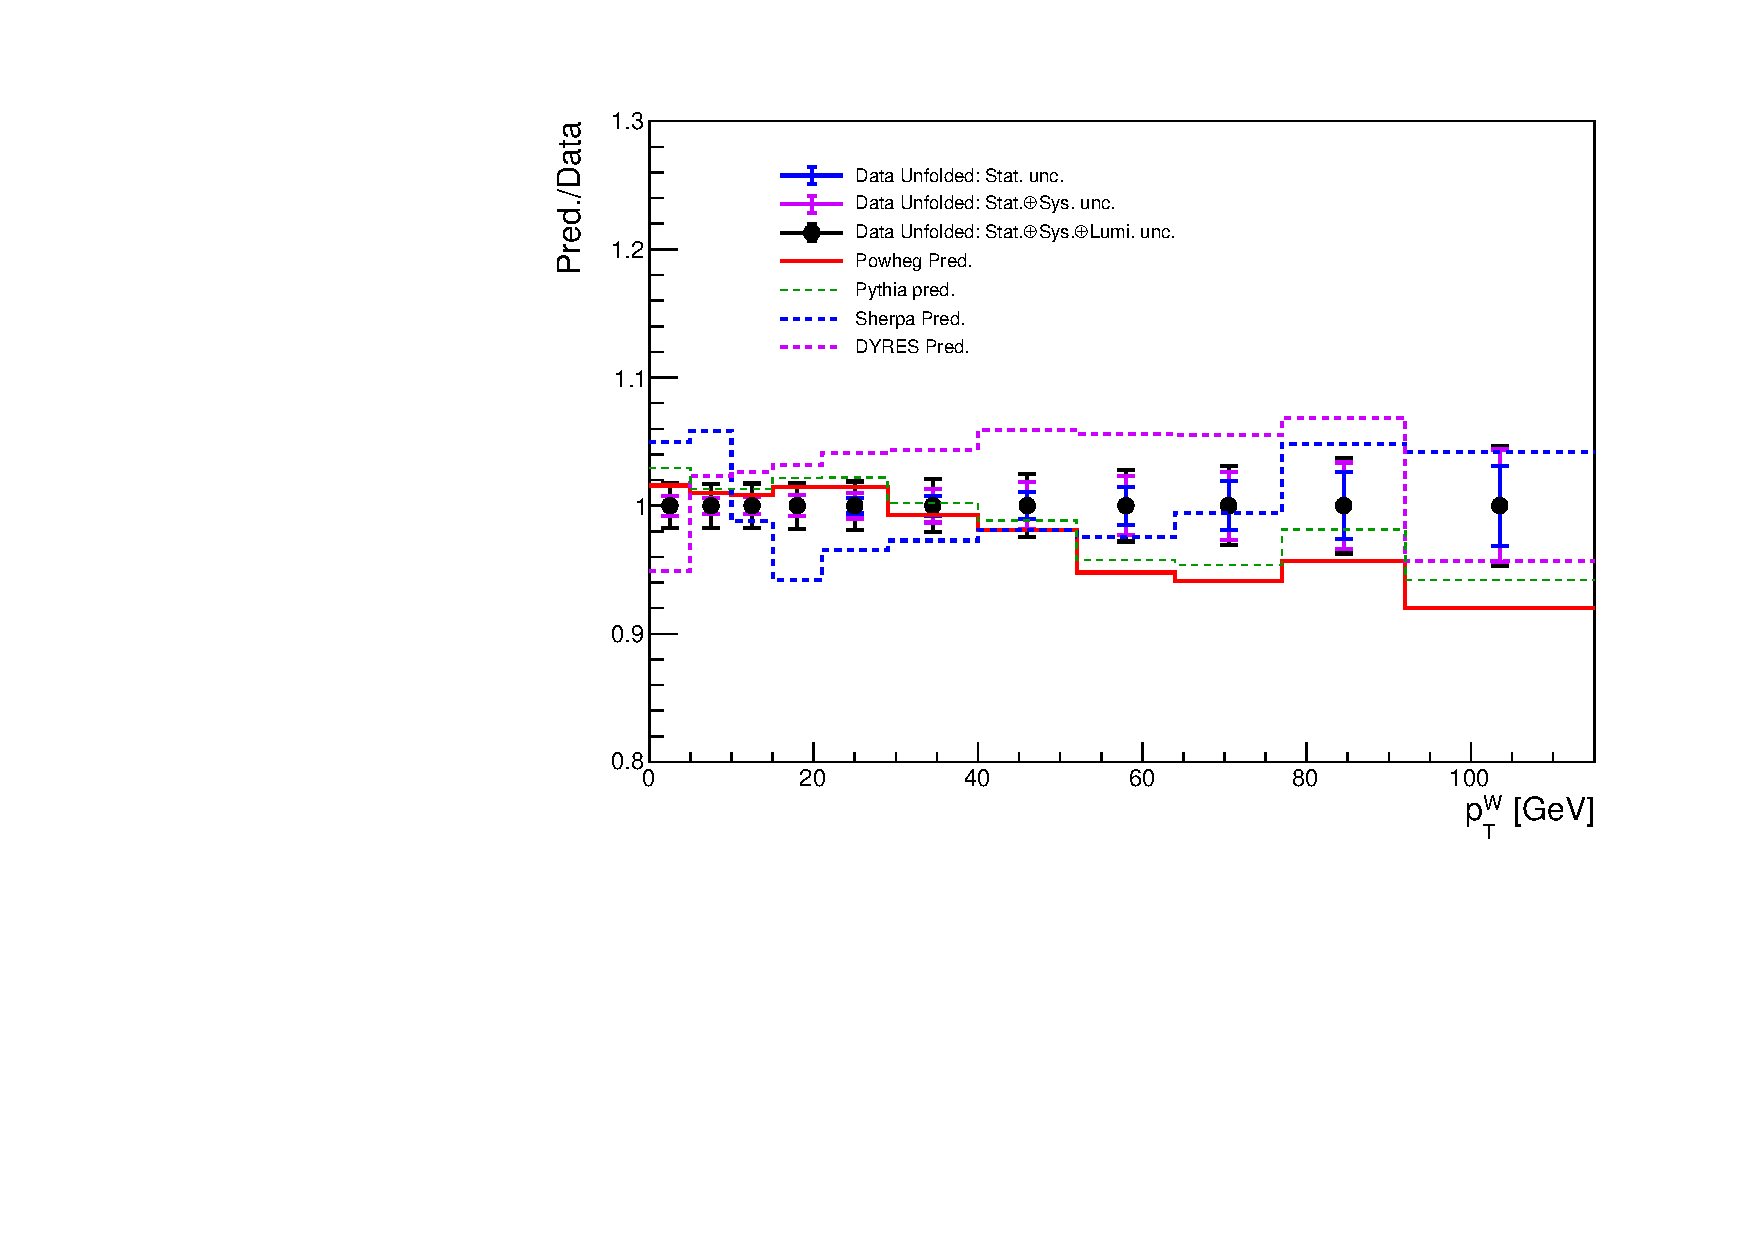
\includegraphics[width=.49\textwidth]{ratio_predictions_Wminusenu_5.pdf}}
	{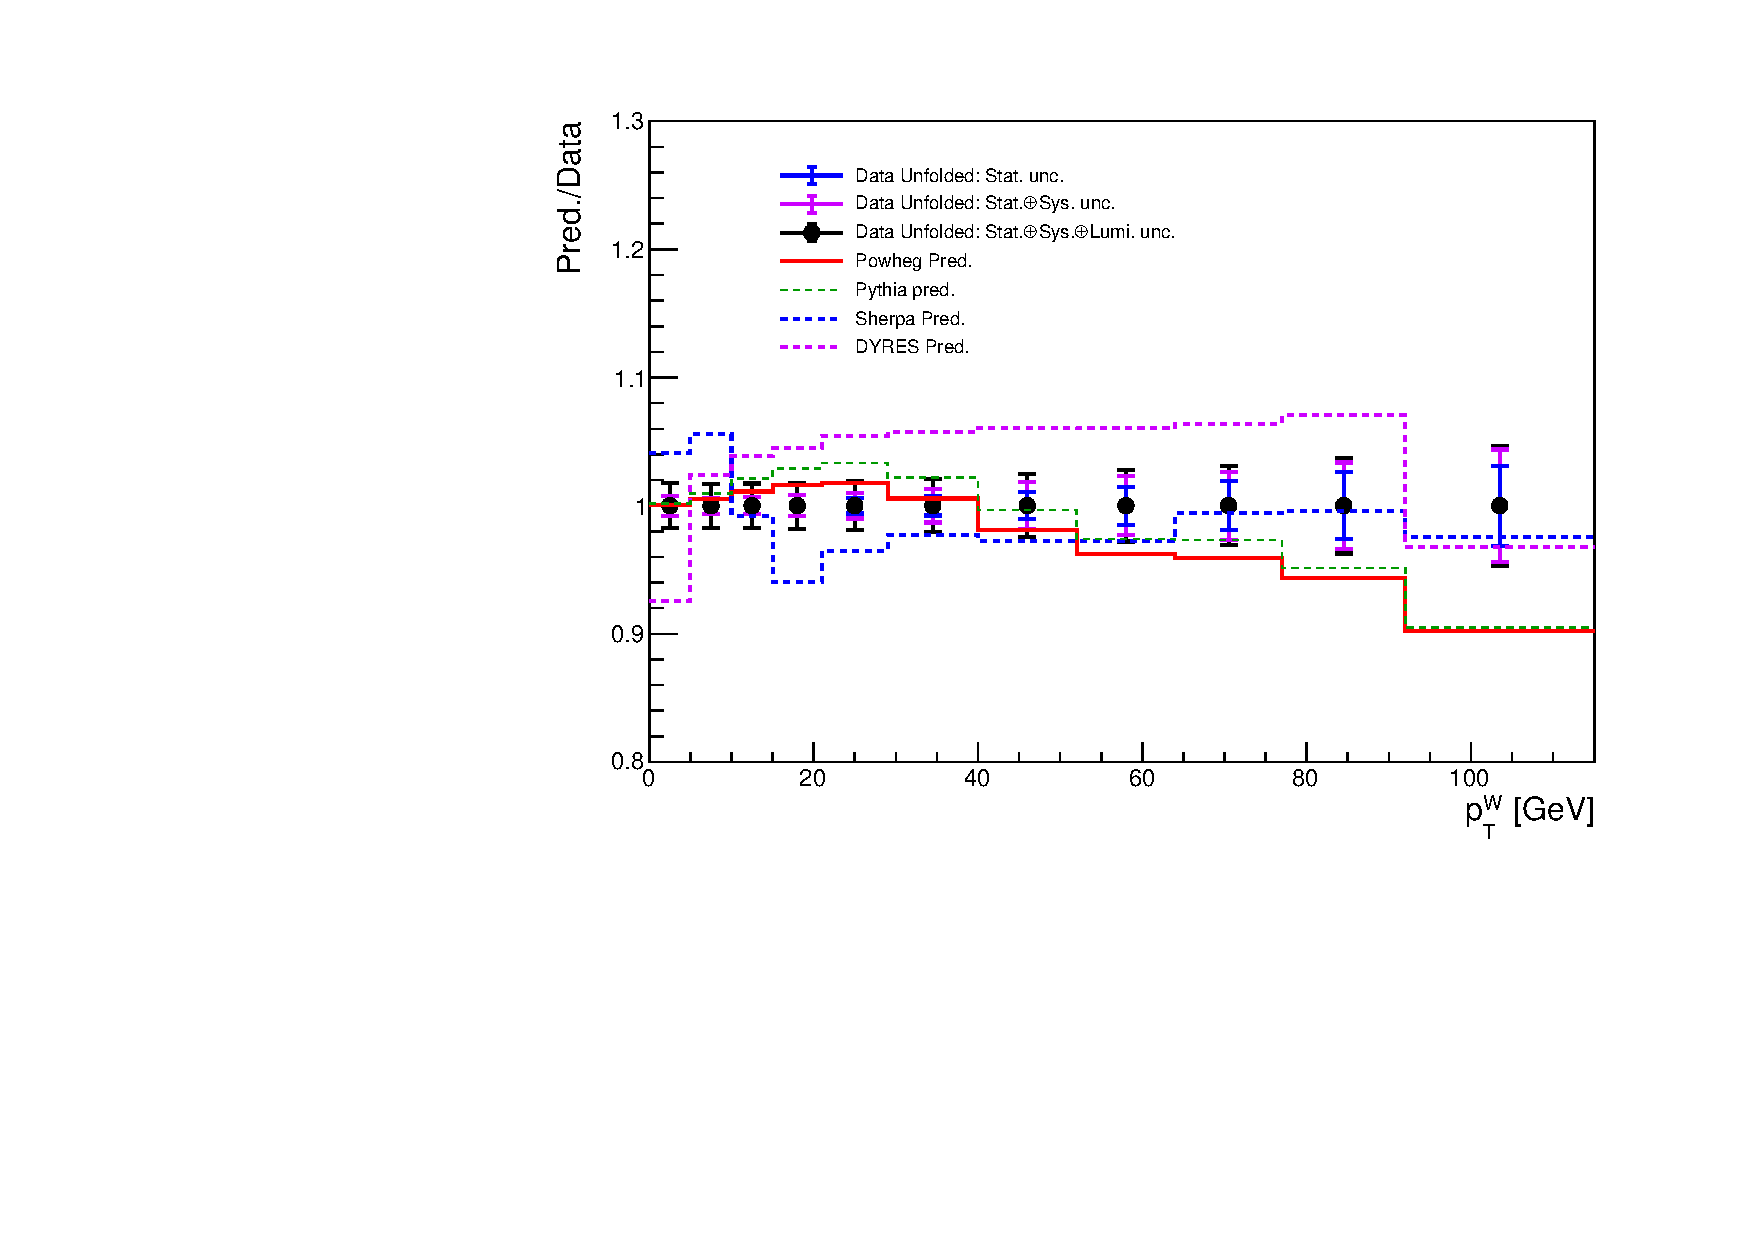
\includegraphics[width=.49\textwidth]{ratio_predictions_Wplusenu_5.pdf}} \\
	{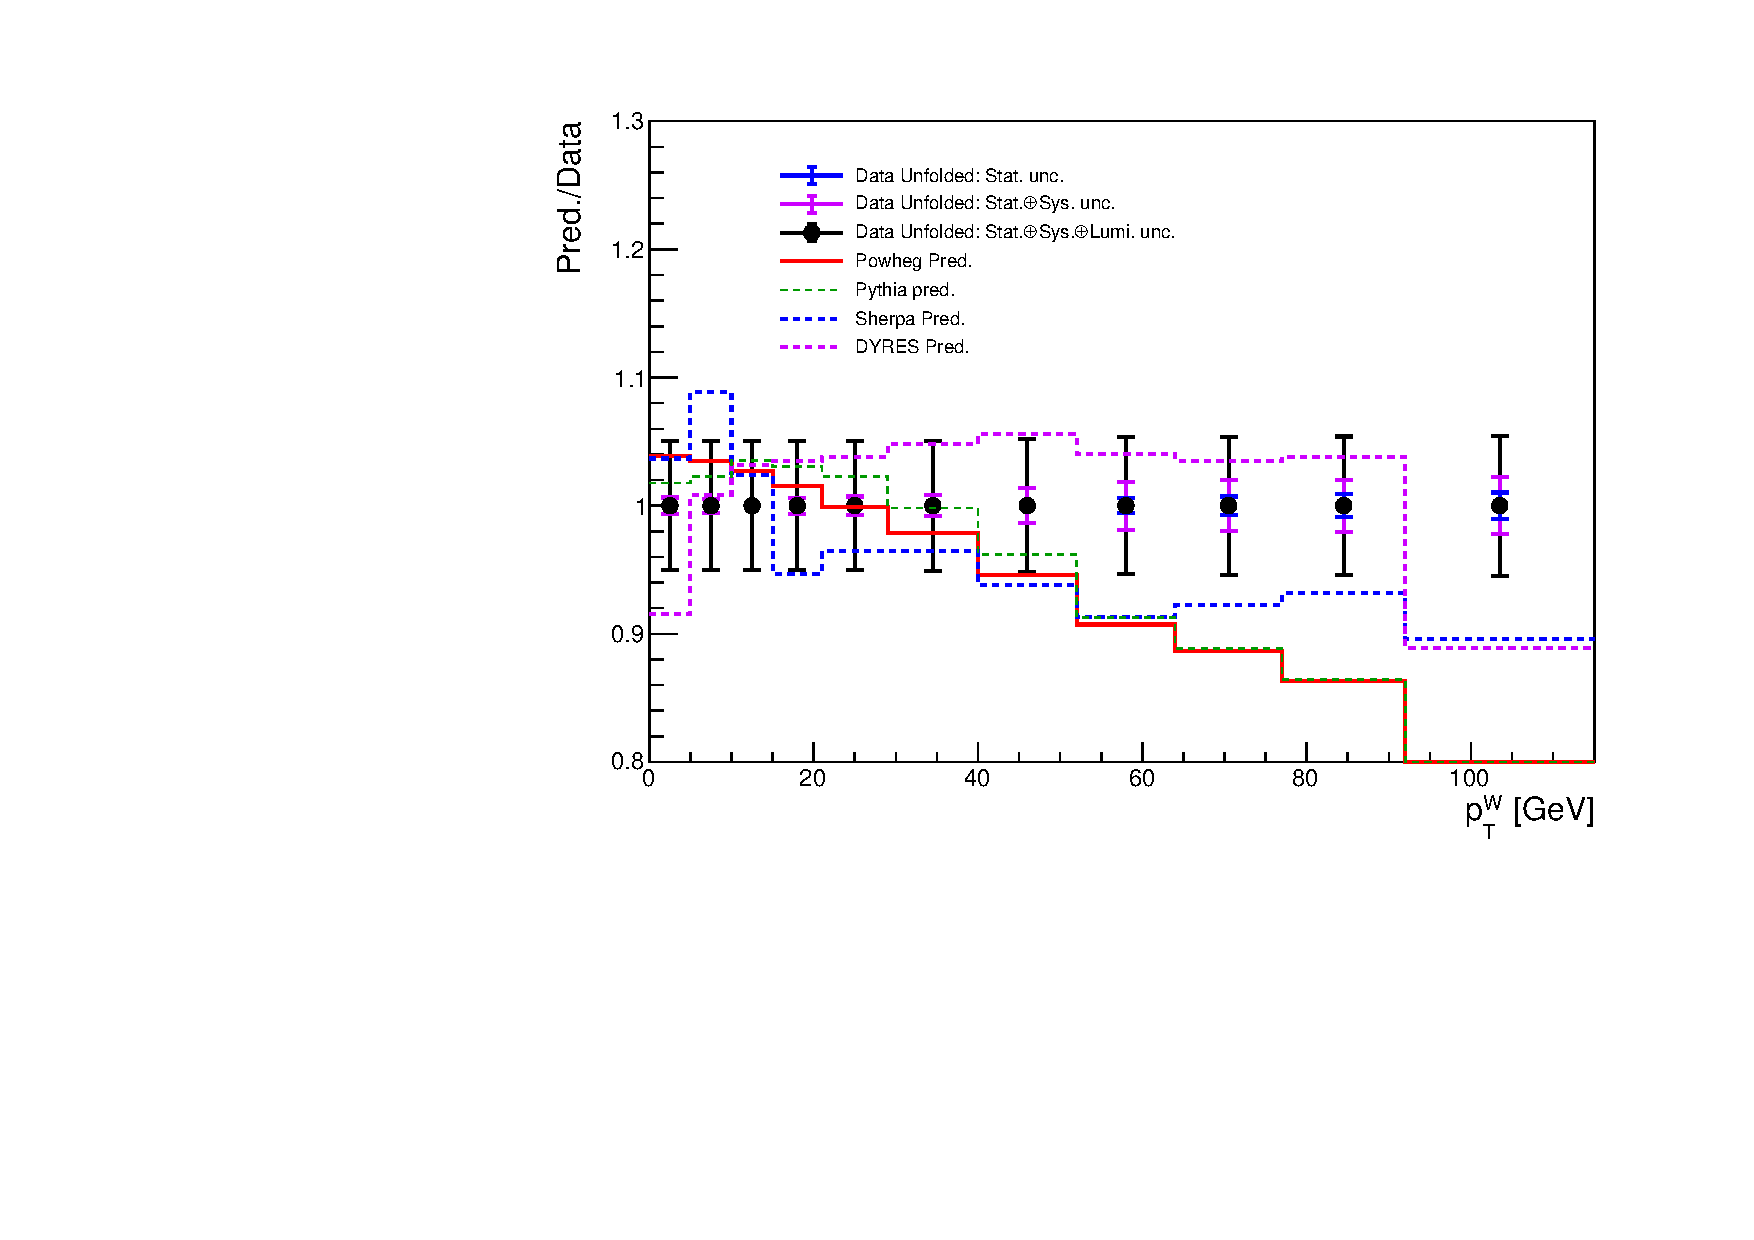
\includegraphics[width=.49\textwidth]{ratio_predictions_Wminusenu_13.pdf}}
	{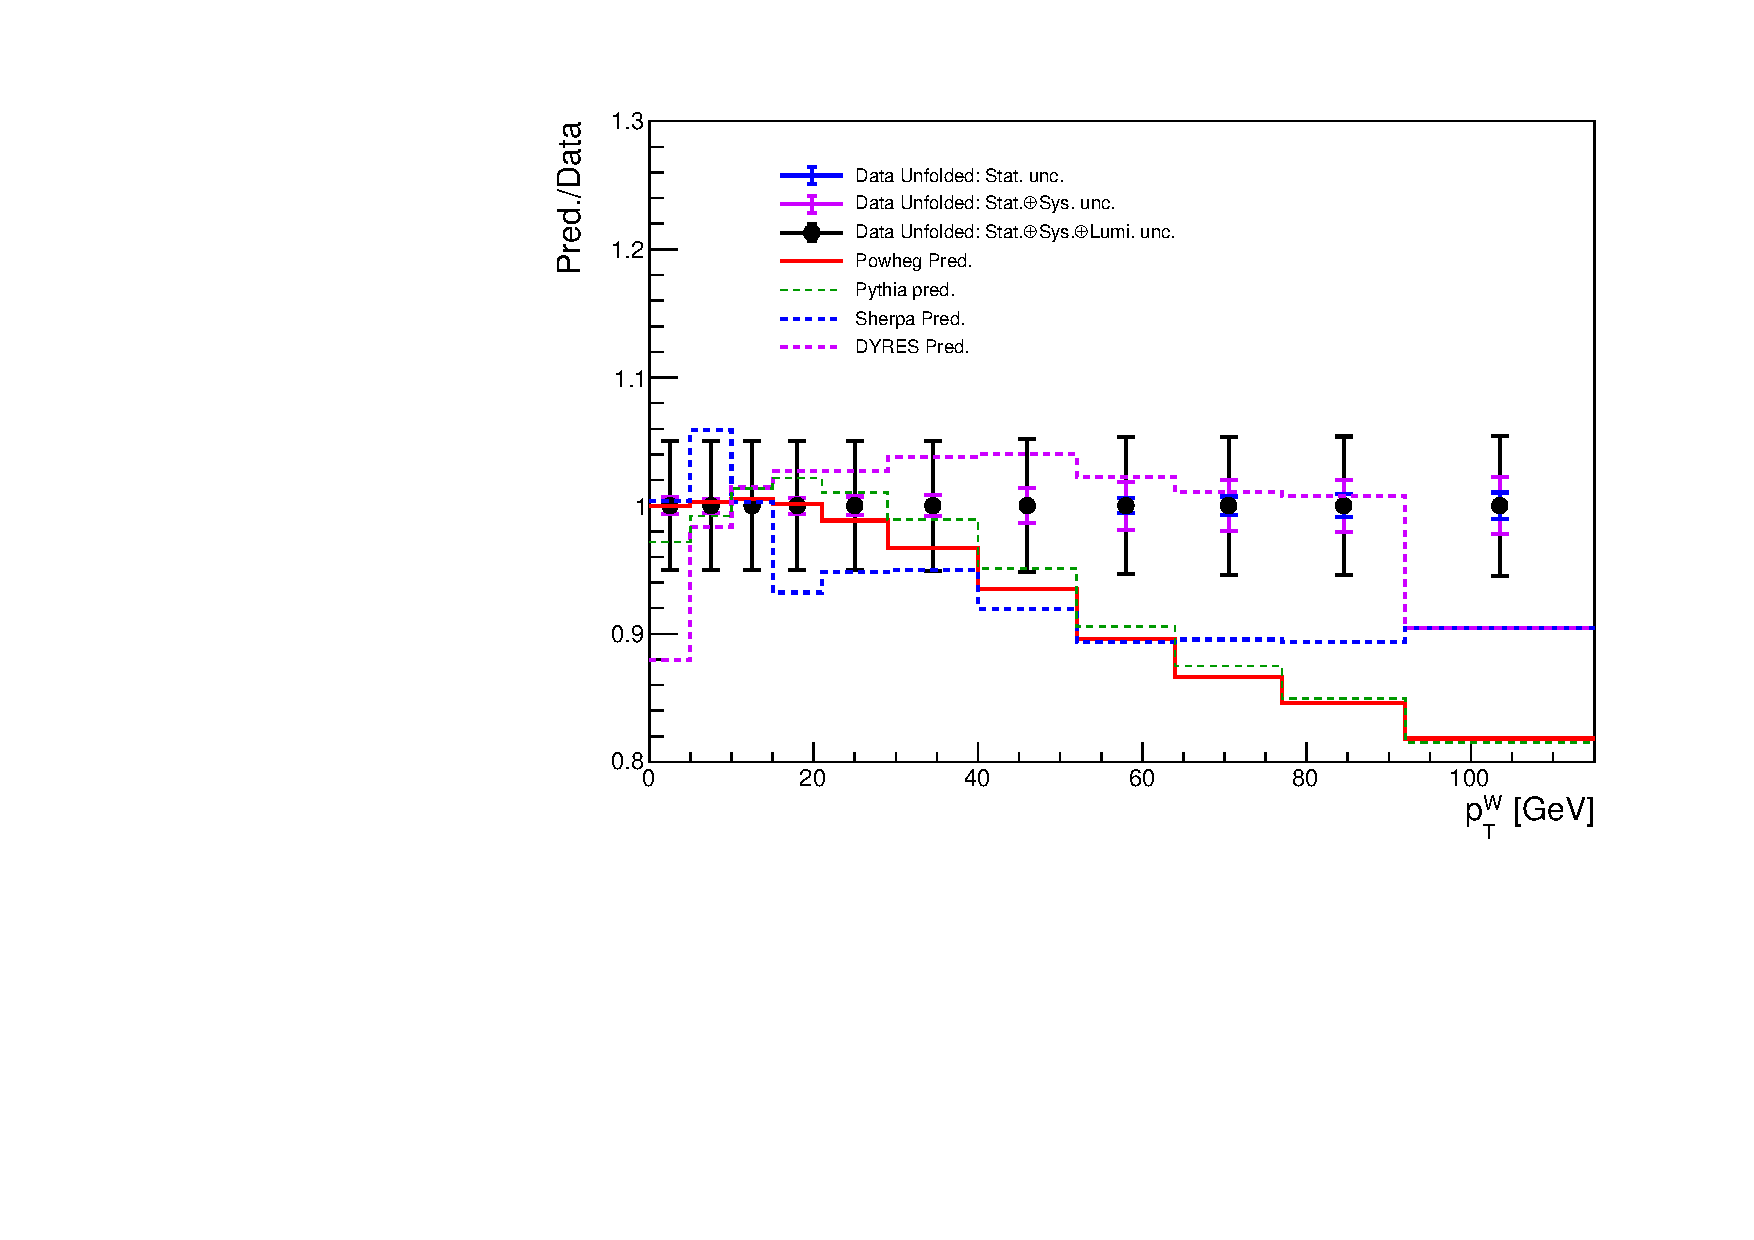
\includegraphics[width=.49\textwidth]{ratio_predictions_Wplusenu_13.pdf}}
	\caption{Unfolded measurement results in the $W^-$ (left) and $W^+$ (right) electron channels, at 5~TeV (top) and 13~TeV (bottom).}
	\label{fig:results_predictions_elec}
\end{figure}

\begin{figure}[h]
	\centering
	{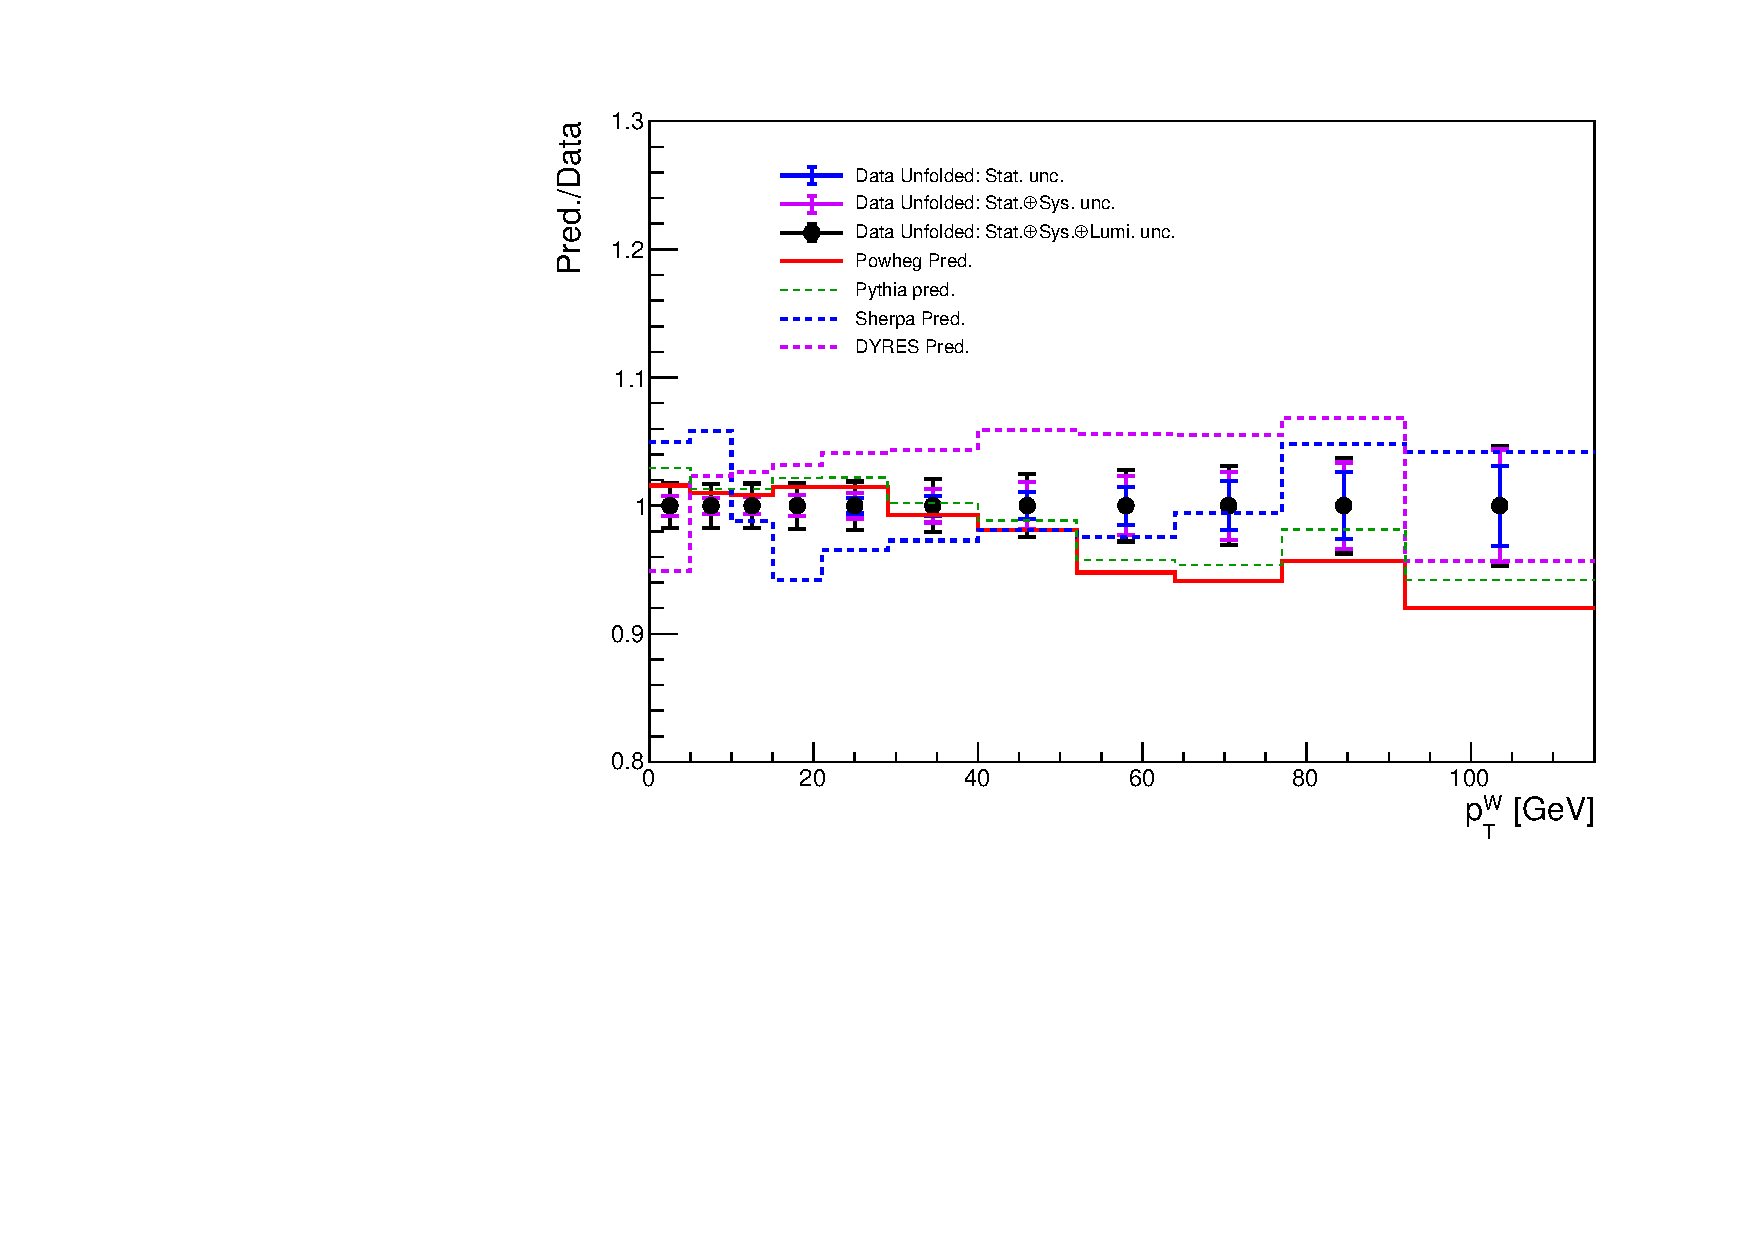
\includegraphics[width=.49\textwidth]{ratio_predictions_Wminusenu_5.pdf}}
	{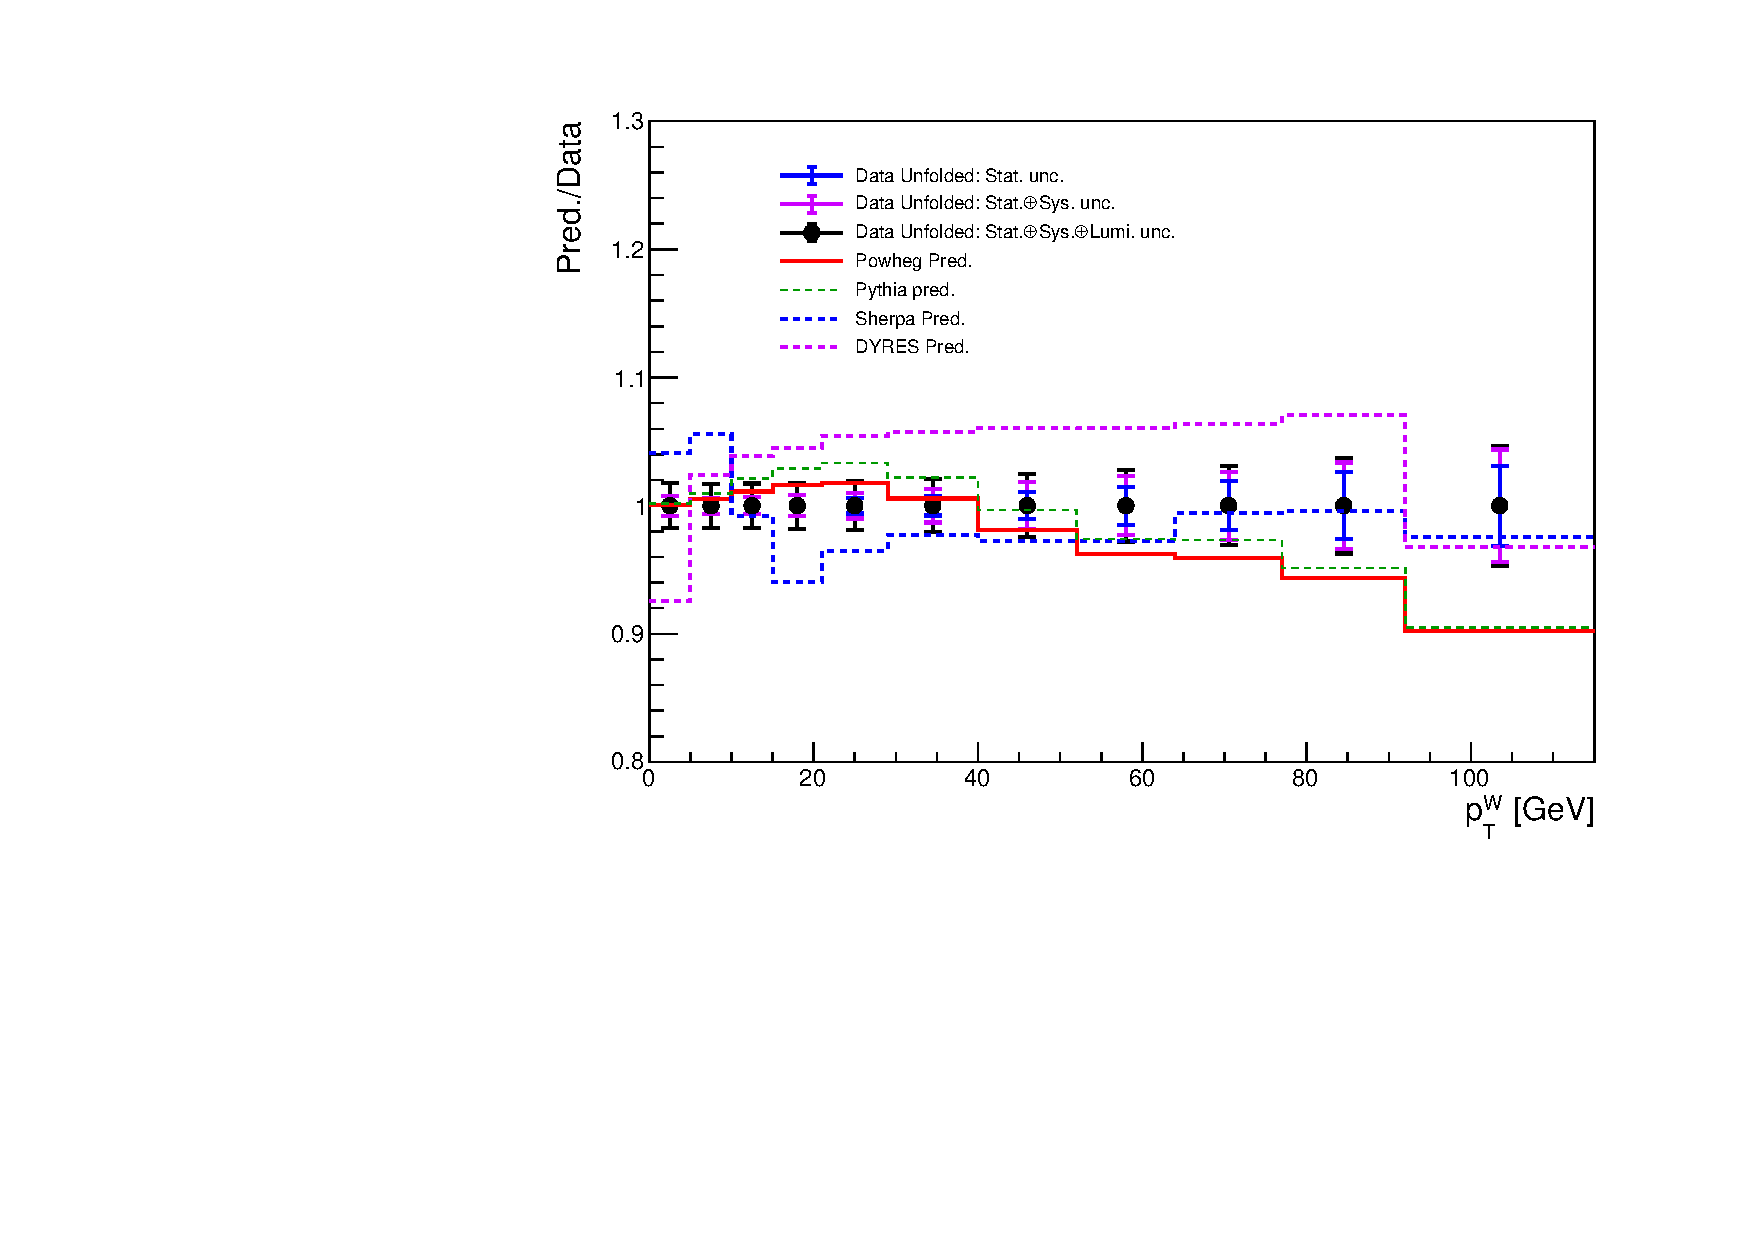
\includegraphics[width=.49\textwidth]{ratio_predictions_Wplusenu_5.pdf}} \\
	{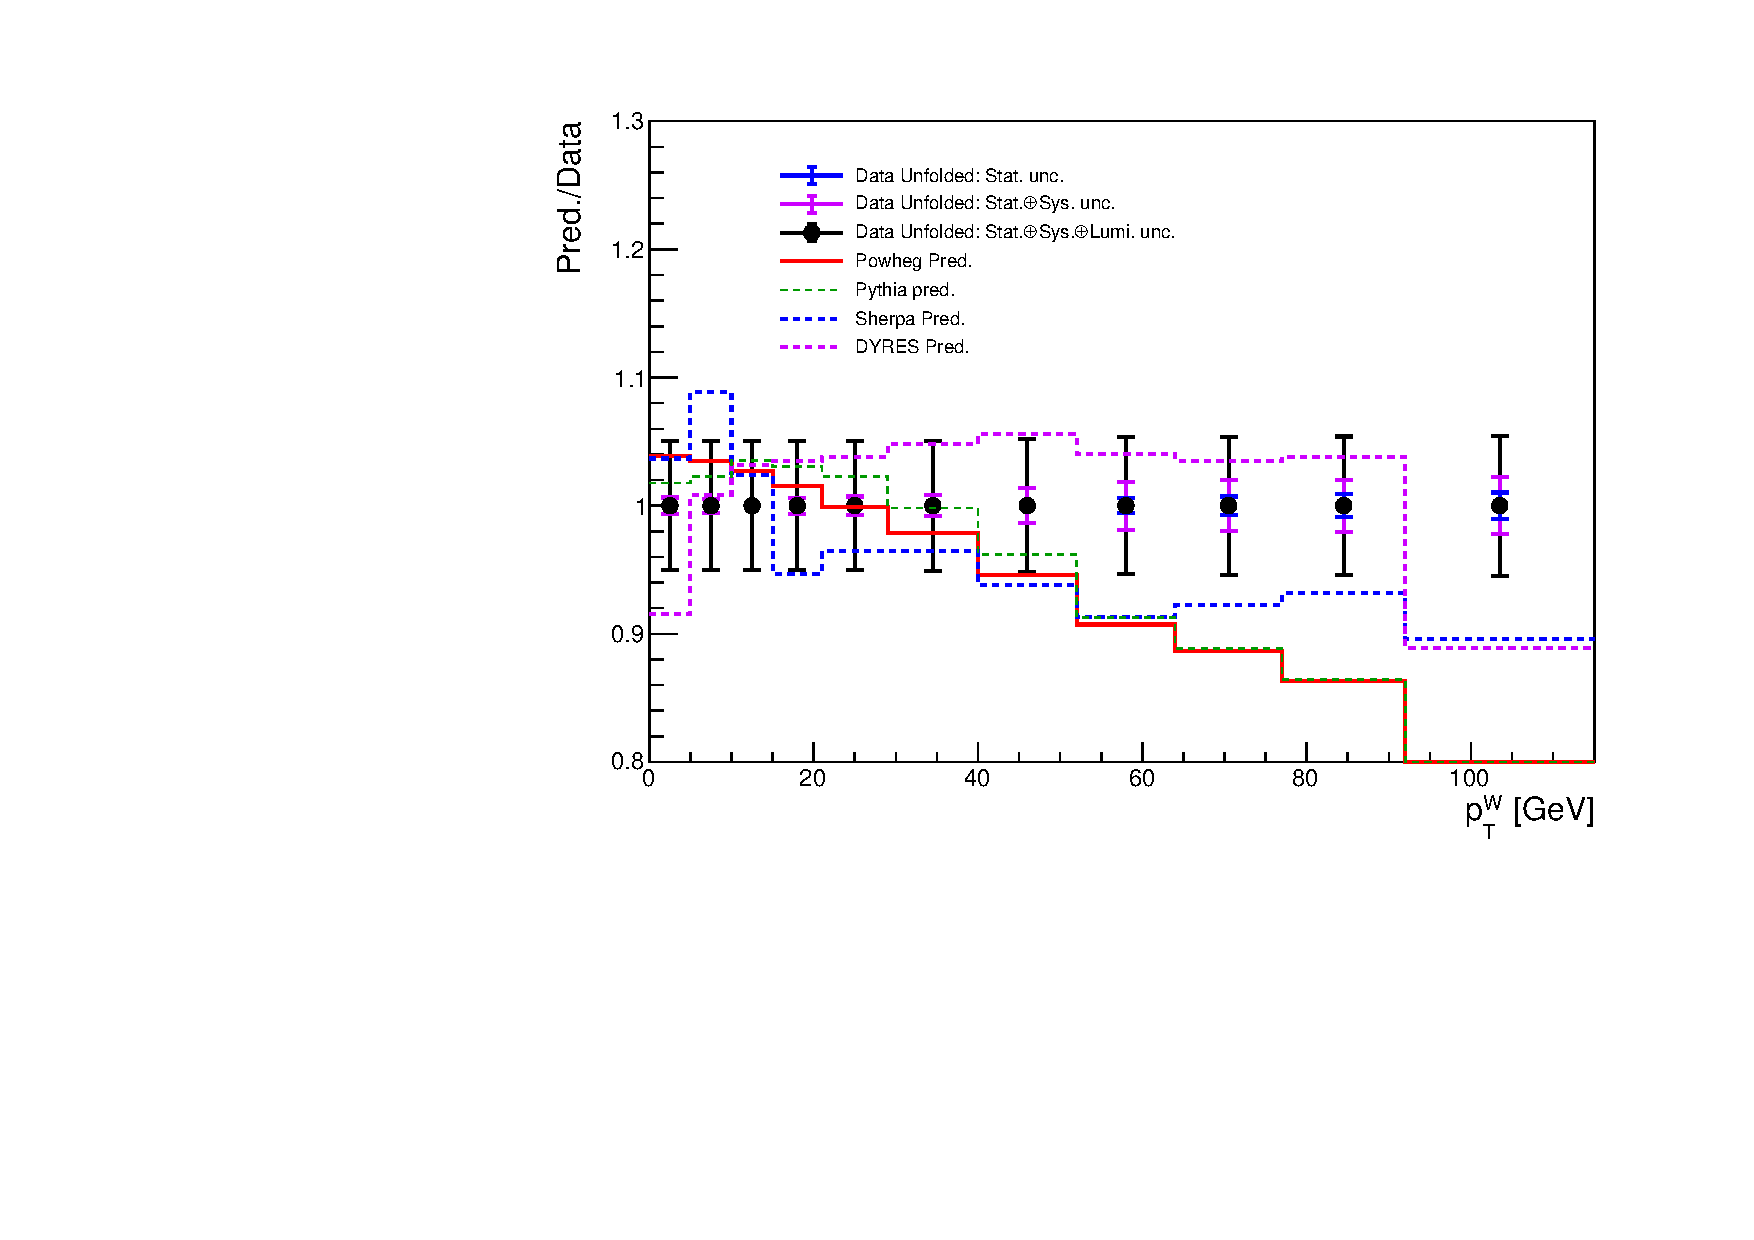
\includegraphics[width=.49\textwidth]{ratio_predictions_Wminusenu_13.pdf}}
	{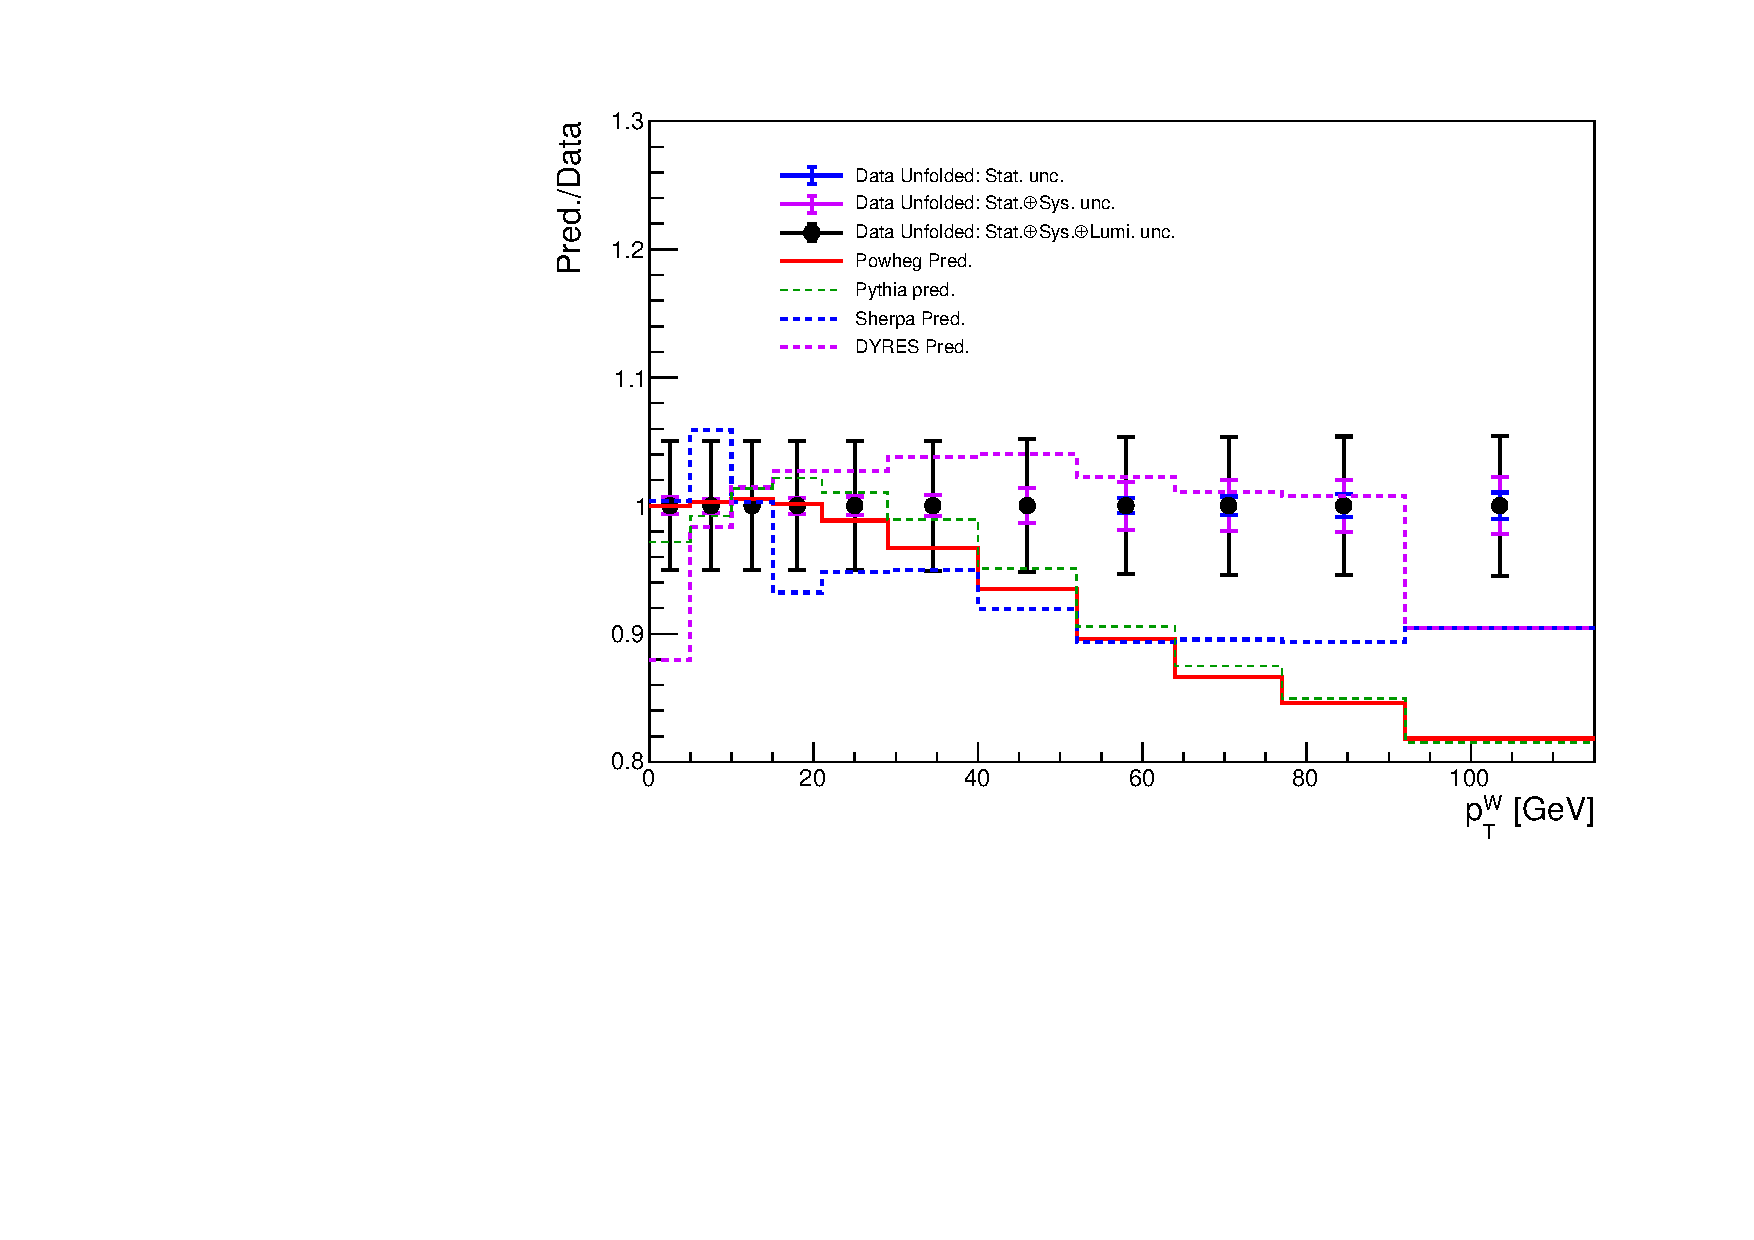
\includegraphics[width=.49\textwidth]{ratio_predictions_Wplusenu_13.pdf}}
	\caption{Unfolded measurement results in the $W^-$ (left) and $W^+$ (right) muon channels, at 5~TeV (top) and 13~TeV (bottom).}
	\label{fig:results_predictions_muon}
\end{figure}